\section{Risultati}

\subsection{Differenze tra gruppi ed effect size}
Le features EEG sono state confrontate tra soggetti ADHD e Control mediante test di Mann-Whitney U. 
Per quantificare la grandezza della differenza tra i gruppi è stato calcolato Cohen's $d$.
 Le prime dieci feature ordinate secondo il valore assoluto di Cohen's $d$ sono riportate nella Tabella~\ref{tab:top10_cohen}.

\begin{table}[H]
	\centering
	\small
	\begin{tabular}{lrrrr}
		\hline
		\textbf{Feature} & \textbf{ADHD mean} & \textbf{Control mean} & \textbf{Cohen's $d$} & \textbf{$p_{FDR}$} \\
		\hline
		\texttt{temporal\_theta\_beta\_ratio} & 1.861 & 2.746 & -0.717 & 0.030 \\
		\texttt{T7\_theta\_beta\_ratio} & 2.206 & 3.402 & -0.657 & 0.039 \\
		\texttt{Pz\_theta\_beta\_ratio} & 2.449 & 3.554 & -0.638 & 0.085 \\
		\texttt{P7\_theta\_beta\_ratio} & 1.364 & 2.097 & -0.596 & 0.039 \\
		\texttt{P7\_theta\_power} & 2262.8 & 4606.1 & -0.585 & 0.039 \\
		\texttt{P7\_delta\_power} & 9224.3 & 27307.8 & -0.562 & 0.030 \\
		\texttt{Pz\_delta\_power} & 11517.6 & 26783.3 & -0.539 & 0.030 \\
		\texttt{parietal\_delta\_power\_mean} & 12388.7 & 25533.5 & -0.534 & 0.191 \\
		\texttt{O1\_theta\_beta\_ratio} & 1.673 & 2.329 & -0.505 & 0.227 \\
		\texttt{occipital\_theta\_beta\_ratio} & 1.477 & 1.980 & -0.484 & 0.233 \\
		\hline
	\end{tabular}
	\caption{Prime dieci feature EEG ordinate secondo il valore assoluto di Cohen's $d$. Valori negativi indicano valori medi più alti nel gruppo Control rispetto al gruppo ADHD.}
	\label{tab:top10_cohen}
\end{table}

Le feature con maggiore effect size sono prevalentemente associate al rapporto theta/beta e alle potenze nelle bande lente, soprattutto in regioni temporali, parietali e occipitali. Tutte le prime dieci feature mostrano Cohen's $d$ negativo, indicando valori medi più elevati nel gruppo Control. 

Per visualizzare la distribuzione spaziale degli effect size, Cohen's $d$ è stato rappresentato sia a livello regionale sia a livello di singolo canale.

\begin{figure}[H]
	\centering
	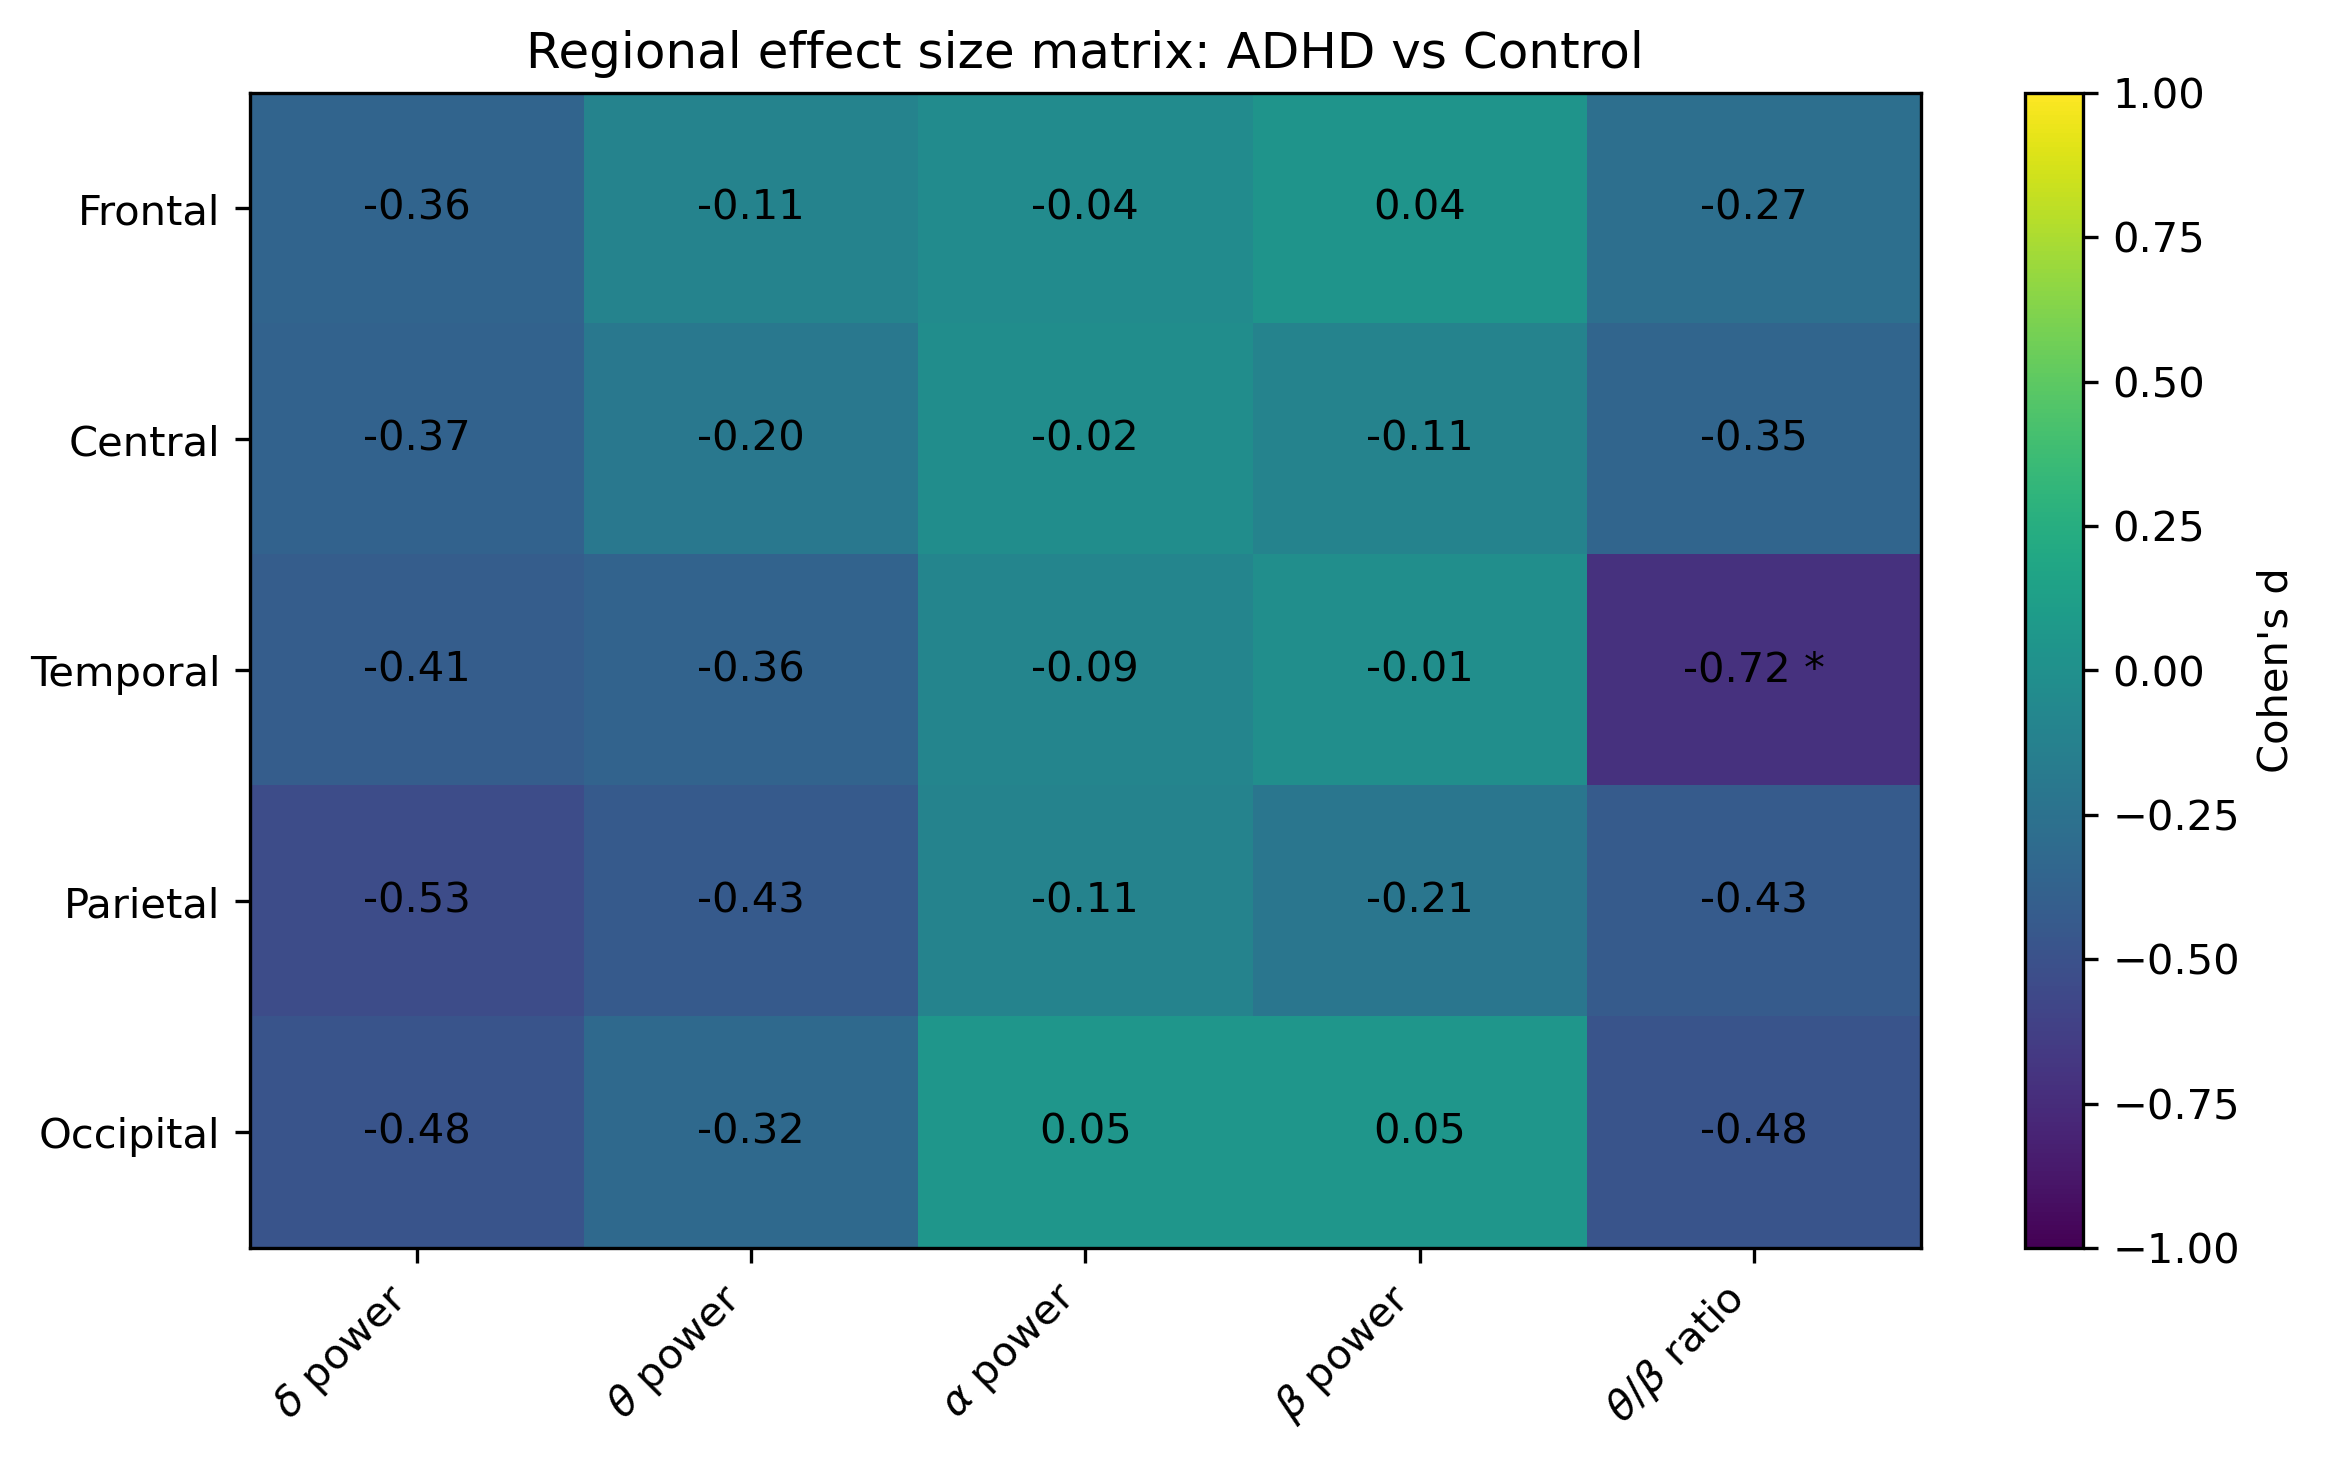
\includegraphics[width=0.85\textwidth]{../figures/1b_regional_effect_size.png}
	\caption{Matrice degli effect size regionali. Ogni cella riporta Cohen's $d$ per una combinazione regione-banda. L'asterisco indica una feature significativa dopo correzione FDR.}
	\label{fig:regional_effect_size}
\end{figure}

Anche matrice regionale mostra effect size prevalentemente negativi, in particolare per la banda delta e per il rapporto theta/beta. Il valore più marcato riguarda il rapporto theta/beta temporale, che risulta anche significativo dopo correzione FDR (contrassegnato con $*$).

\begin{figure}[H]
	\centering
	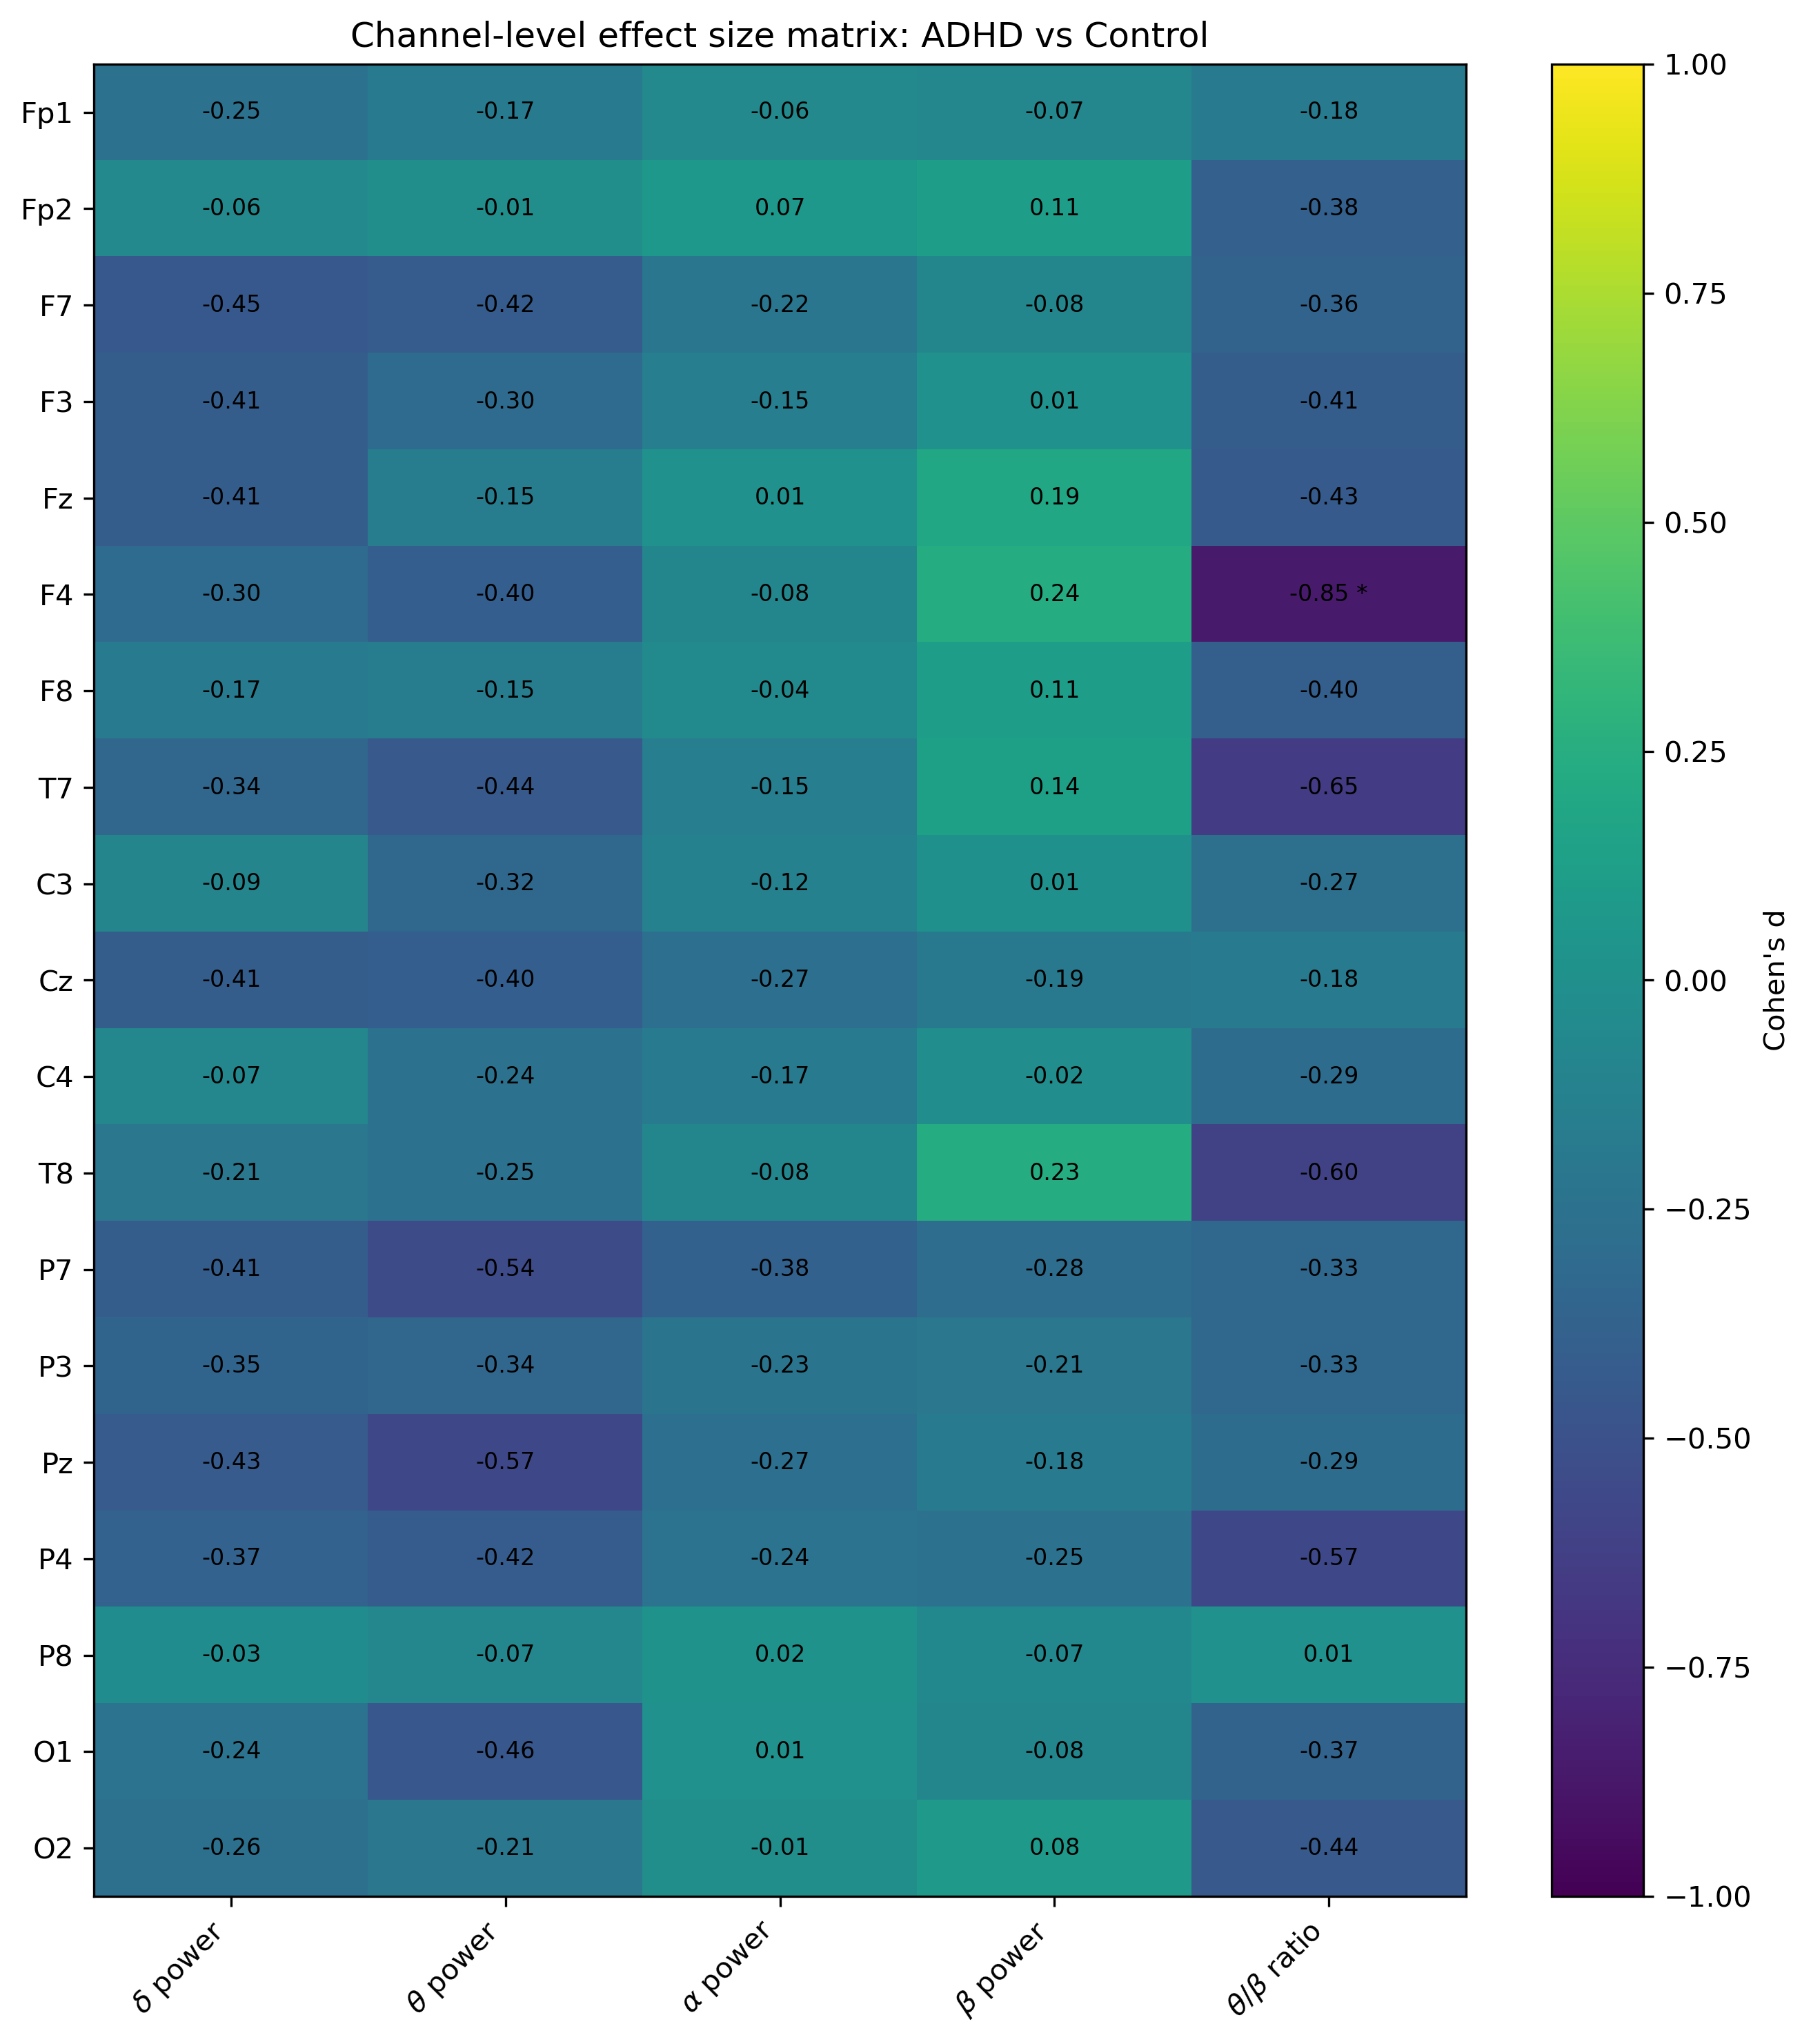
\includegraphics[width=0.85\textwidth]{../figures/1b_Tchannel_effect_size.png}
	\caption{Matrice degli effect size a livello di singolo canale. Ogni cella riporta Cohen's $d$ per una combinazione canale-banda. L'asterisco indica una feature significativa dopo correzione FDR.}
	\label{fig:channel_effect_size}
\end{figure}

La matrice canale-livello evidenzia che le differenze più marcate si concentrano soprattutto nei canali temporali e parietali, in particolare per il rapporto theta/beta e per le potenze delta e theta. La rappresentazione a singolo canale conserva maggiore dettaglio spaziale, mentre la rappresentazione regionale fornisce una sintesi più compatta.

\subsection{Feature significative dopo correzione FDR}

Per controllare il problema dei confronti multipli, i p-value ottenuti dai test di Mann-Whitney U sono stati corretti mediante procedura Benjamini-Hochberg. Le feature con $p_{FDR} < 0.05$ sono state considerate statisticamente significative dopo correzione. I risultati sono riportati nella Tabella~\ref{tab:fdr_features} e visualizzati in Figura~\ref{fig:fdr_features_boxplot}.

\begin{table}[H]
	\centering
	\small
	\begin{tabular}{lrrrr}
		\hline
		\textbf{Feature} & \textbf{ADHD mean} & \textbf{Control mean} & \textbf{Cohen's $d$} & \textbf{$p_{FDR}$} \\
		\hline
		\texttt{temporal\_theta\_beta\_ratio} & 1.861 & 2.746 & -0.717 & 0.030 \\
		\texttt{P7\_delta\_power} & 9224.3 & 27307.8 & -0.562 & 0.030 \\
		\texttt{Pz\_delta\_power} & 11517.6 & 26783.3 & -0.539 & 0.030 \\
		\texttt{T7\_theta\_beta\_ratio} & 2.206 & 3.402 & -0.657 & 0.039 \\
		\texttt{P7\_theta\_beta\_ratio} & 1.364 & 2.097 & -0.596 & 0.039 \\
		\texttt{P7\_theta\_power} & 2262.8 & 4606.1 & -0.585 & 0.039 \\
		\texttt{F4\_beta\_power} & 2417.5 & 2254.9 & 0.060 & 0.039 \\
		\hline
	\end{tabular}
	\caption{Feature EEG risultate significative dopo correzione FDR.}
	\label{tab:fdr_features}
\end{table}

Le feature significative dopo correzione FDR confermano il coinvolgimento del rapporto theta/beta e delle bande lente in canali temporali e parietali. La maggior parte di queste feature presenta Cohen's $d$ negativo, quindi valori medi più elevati nel gruppo Control. L'unica feature significativa con effect size positivo è \texttt{F4\_beta\_power}; tuttavia, il valore di Cohen's $d$ è molto piccolo.

\begin{figure}[H]
	\centering
	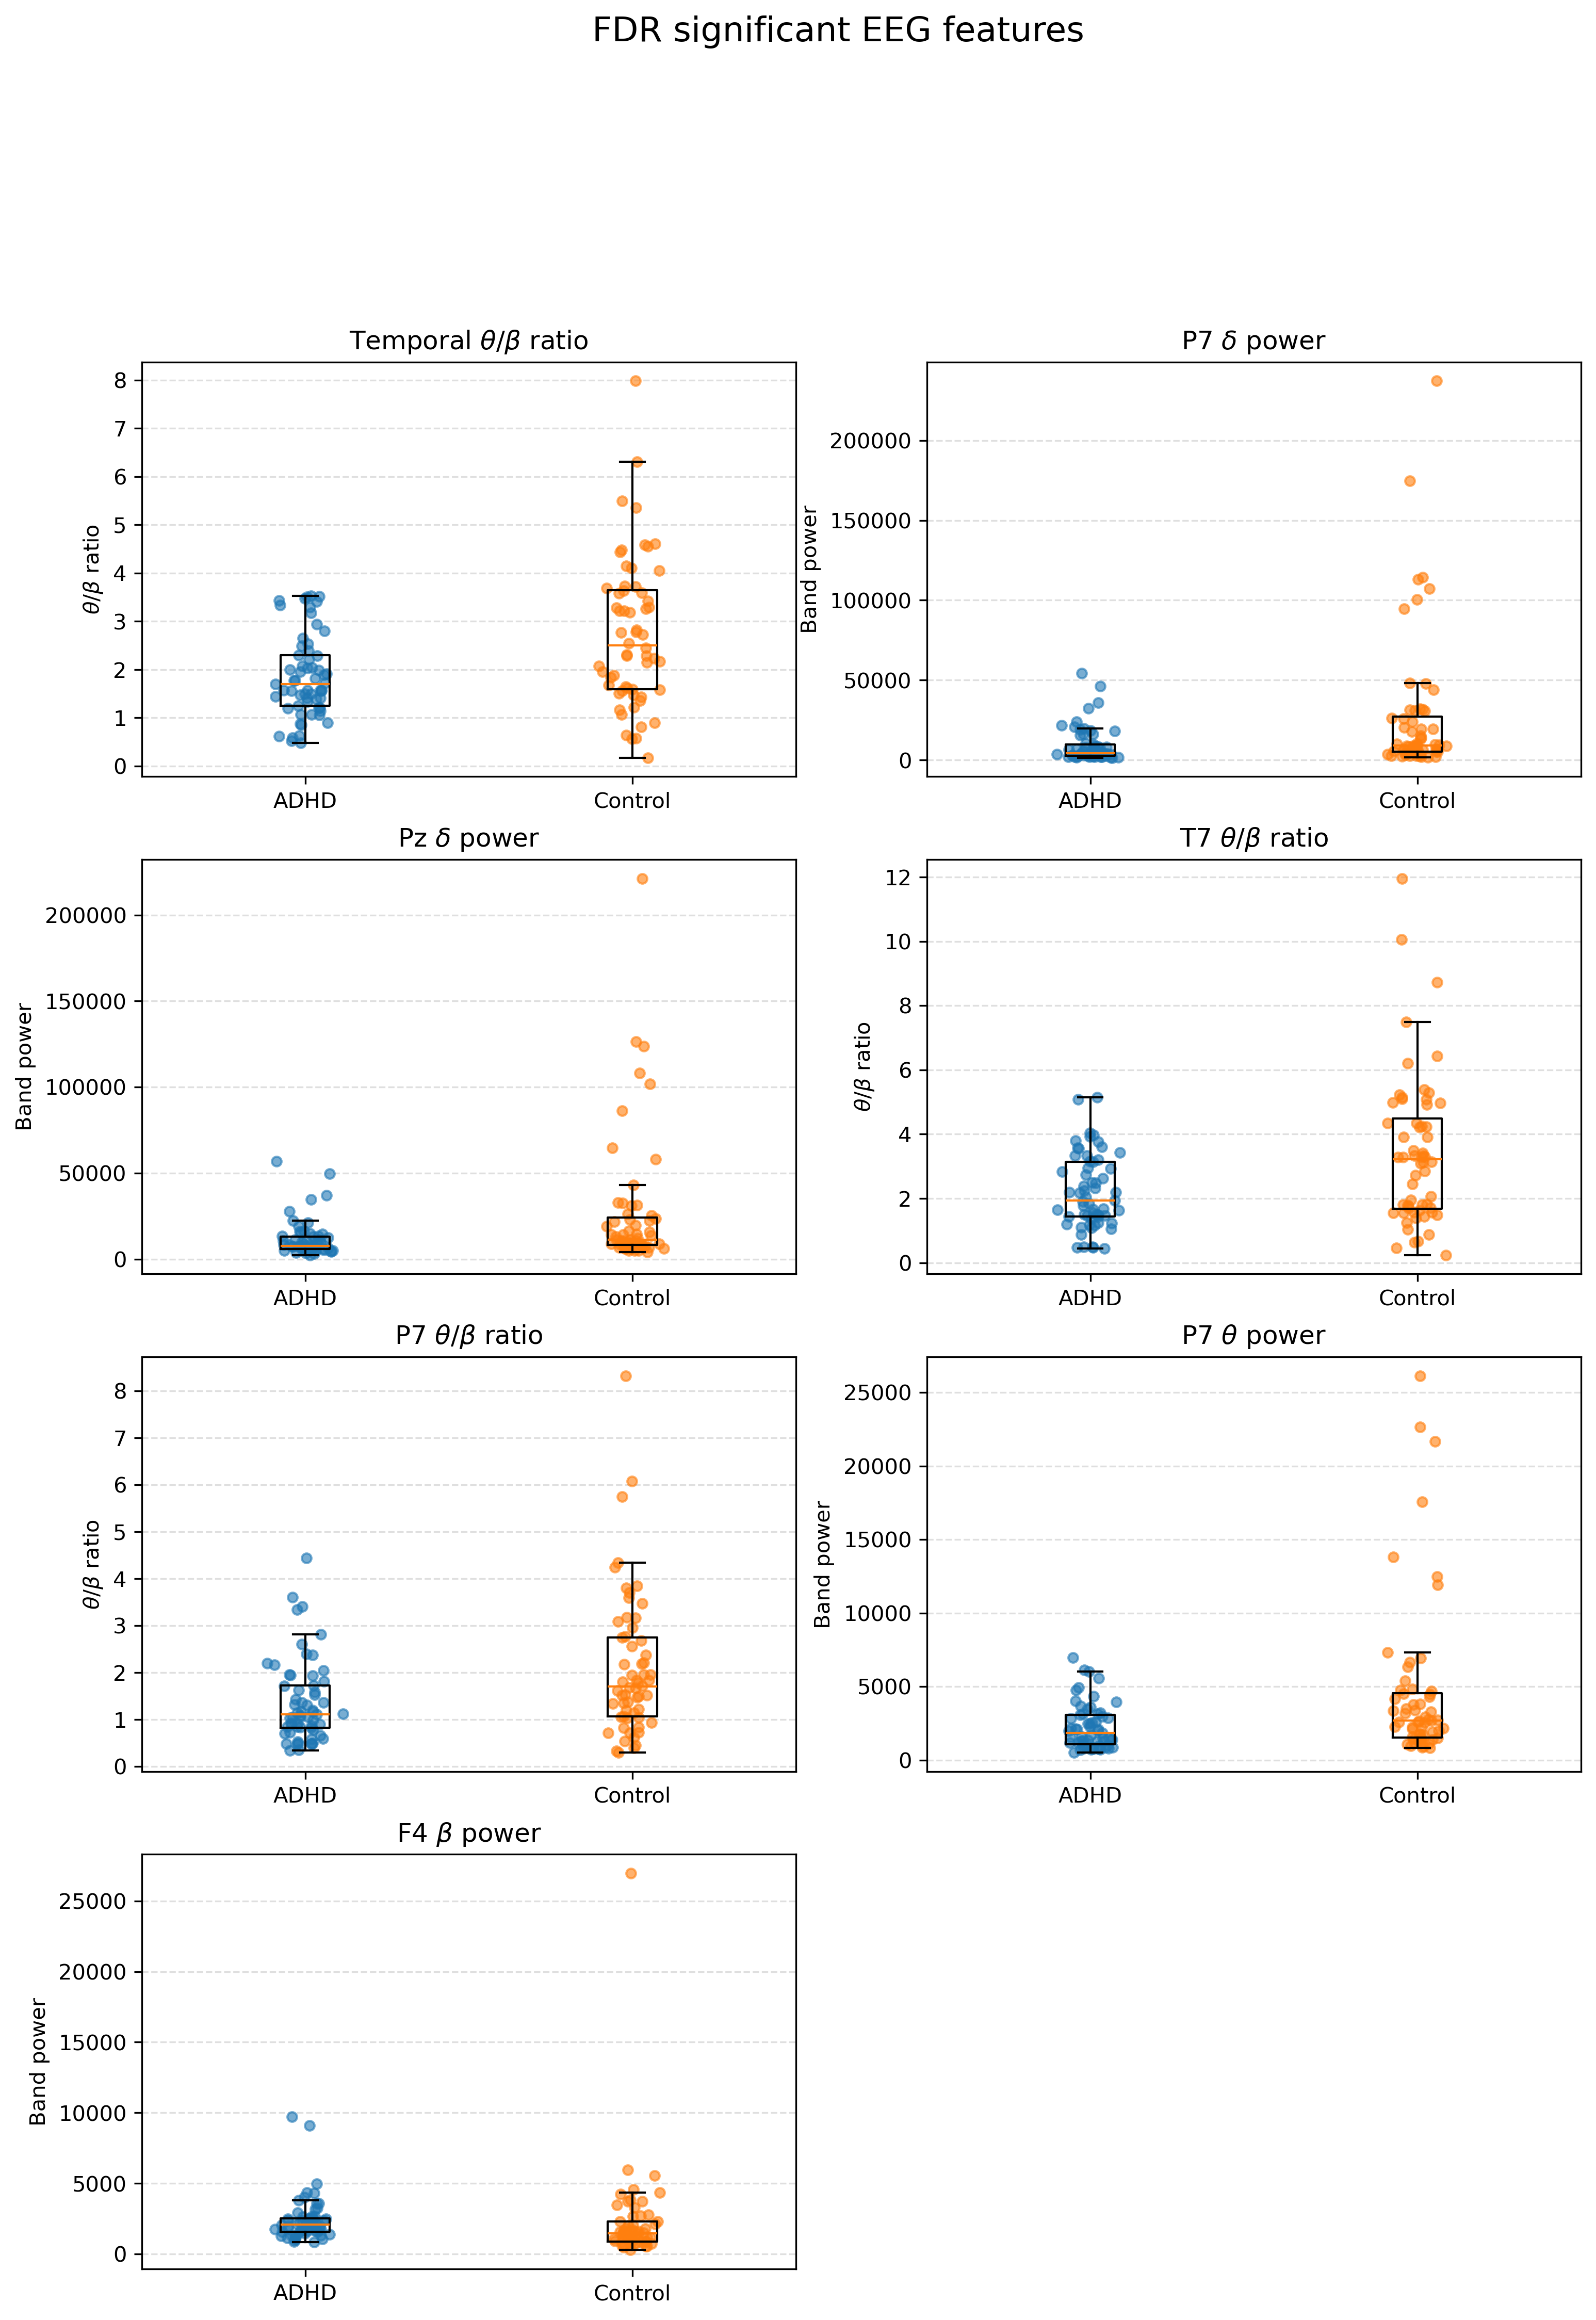
\includegraphics[width=0.95\textwidth]{../figures/1b_FDR_significant_features.png}
	\caption{Distribuzione delle feature EEG significative dopo correzione FDR.}
	\label{fig:fdr_features_boxplot}
\end{figure}


\subsection{Correlazione tra feature}

Per valutare la ridondanza tra feature EEG, sono state calcolate correlazioni di Spearman separatamente nei gruppi ADHD e Control. L'analisi è stata condotta sia sulle feature canale-livello sia sulle feature regionali.

\subsubsection{Correlazioni canale-livello}

Le correlazioni più forti tra feature canale-livello sono riportate nella Tabella~\ref{tab:top_channel_correlations}. Sono state selezionate le dieci correlazioni più forti in valore assoluto per ciascun gruppo.

\begin{table}[H]
	\centering
	\scriptsize
	\begin{tabular}{lllr}
		\hline
		\textbf{Gruppo} & \textbf{Feature 1} & \textbf{Feature 2} & \textbf{$\rho$} \\
		\hline
		ADHD & \texttt{F3\_alpha\_power} & \texttt{Fz\_alpha\_power} & 0.938 \\
		ADHD & \texttt{F3\_beta\_power} & \texttt{Fz\_beta\_power} & 0.917 \\
		ADHD & \texttt{P3\_theta\_beta\_ratio} & \texttt{Pz\_theta\_beta\_ratio} & 0.912 \\
		ADHD & \texttt{P3\_beta\_power} & \texttt{Pz\_beta\_power} & 0.907 \\
		ADHD & \texttt{P3\_theta\_power} & \texttt{Pz\_theta\_power} & 0.905 \\
		ADHD & \texttt{F3\_theta\_power} & \texttt{Fz\_theta\_power} & 0.885 \\
		ADHD & \texttt{P4\_beta\_power} & \texttt{Cz\_beta\_power} & 0.881 \\
		ADHD & \texttt{O2\_delta\_power} & \texttt{O2\_theta\_power} & 0.876 \\
		ADHD & \texttt{P8\_delta\_power} & \texttt{P8\_theta\_power} & 0.874 \\
		ADHD & \texttt{F4\_beta\_power} & \texttt{C4\_beta\_power} & 0.871 \\
		\hline
		Control & \texttt{F3\_theta\_power} & \texttt{C3\_theta\_power} & 0.940 \\
		Control & \texttt{F3\_alpha\_power} & \texttt{Fz\_alpha\_power} & 0.937 \\
		Control & \texttt{F3\_theta\_power} & \texttt{Fz\_theta\_power} & 0.930 \\
		Control & \texttt{F4\_delta\_power} & \texttt{Cz\_delta\_power} & 0.926 \\
		Control & \texttt{O1\_delta\_power} & \texttt{P7\_delta\_power} & 0.919 \\
		Control & \texttt{F3\_beta\_power} & \texttt{Fz\_beta\_power} & 0.918 \\
		Control & \texttt{C3\_delta\_power} & \texttt{Pz\_delta\_power} & 0.909 \\
		Control & \texttt{C4\_theta\_power} & \texttt{Cz\_theta\_power} & 0.909 \\
		Control & \texttt{C3\_theta\_power} & \texttt{P3\_theta\_power} & 0.906 \\
		Control & \texttt{P3\_delta\_power} & \texttt{Pz\_delta\_power} & 0.905 \\
		\hline
	\end{tabular}
	\caption{Dieci correlazioni di Spearman più forti in valore assoluto tra feature canale-livello, calcolate separatamente nei gruppi ADHD e Control.}
	\label{tab:top_channel_correlations}
\end{table}

Le correlazioni canale-livello più forti in valore assoluto risultano tutte positive in entrambi i gruppi. Questo indica che le principali ridondanze tra feature derivano soprattutto da potenze della stessa banda o da feature spettrali simili misurate in canali vicini. Nel gruppo ADHD compaiono correlazioni elevate tra canali frontali e parietali, come \texttt{F3}--\texttt{Fz} e \texttt{P3}--\texttt{Pz}. Nel gruppo Control si osservano correlazioni molto alte tra canali frontali, centrali e parietali, in particolare per le bande theta, alpha, beta e delta. Questa struttura conferma che molte feature canale-livello non sono indipendenti, ma descrivono pattern spettrali parzialmente sovrapposti.

\subsubsection{Correlazioni regionali}

Le matrici di correlazione tra feature regionali sono mostrate in Figura~\ref{fig:regional_corr_matrix_by_group}. Le dieci correlazioni regionali più forti in valore assoluto sono riportate nella Tabella~\ref{tab:top_regional_correlations}.

\begin{figure}[H]
	\centering
	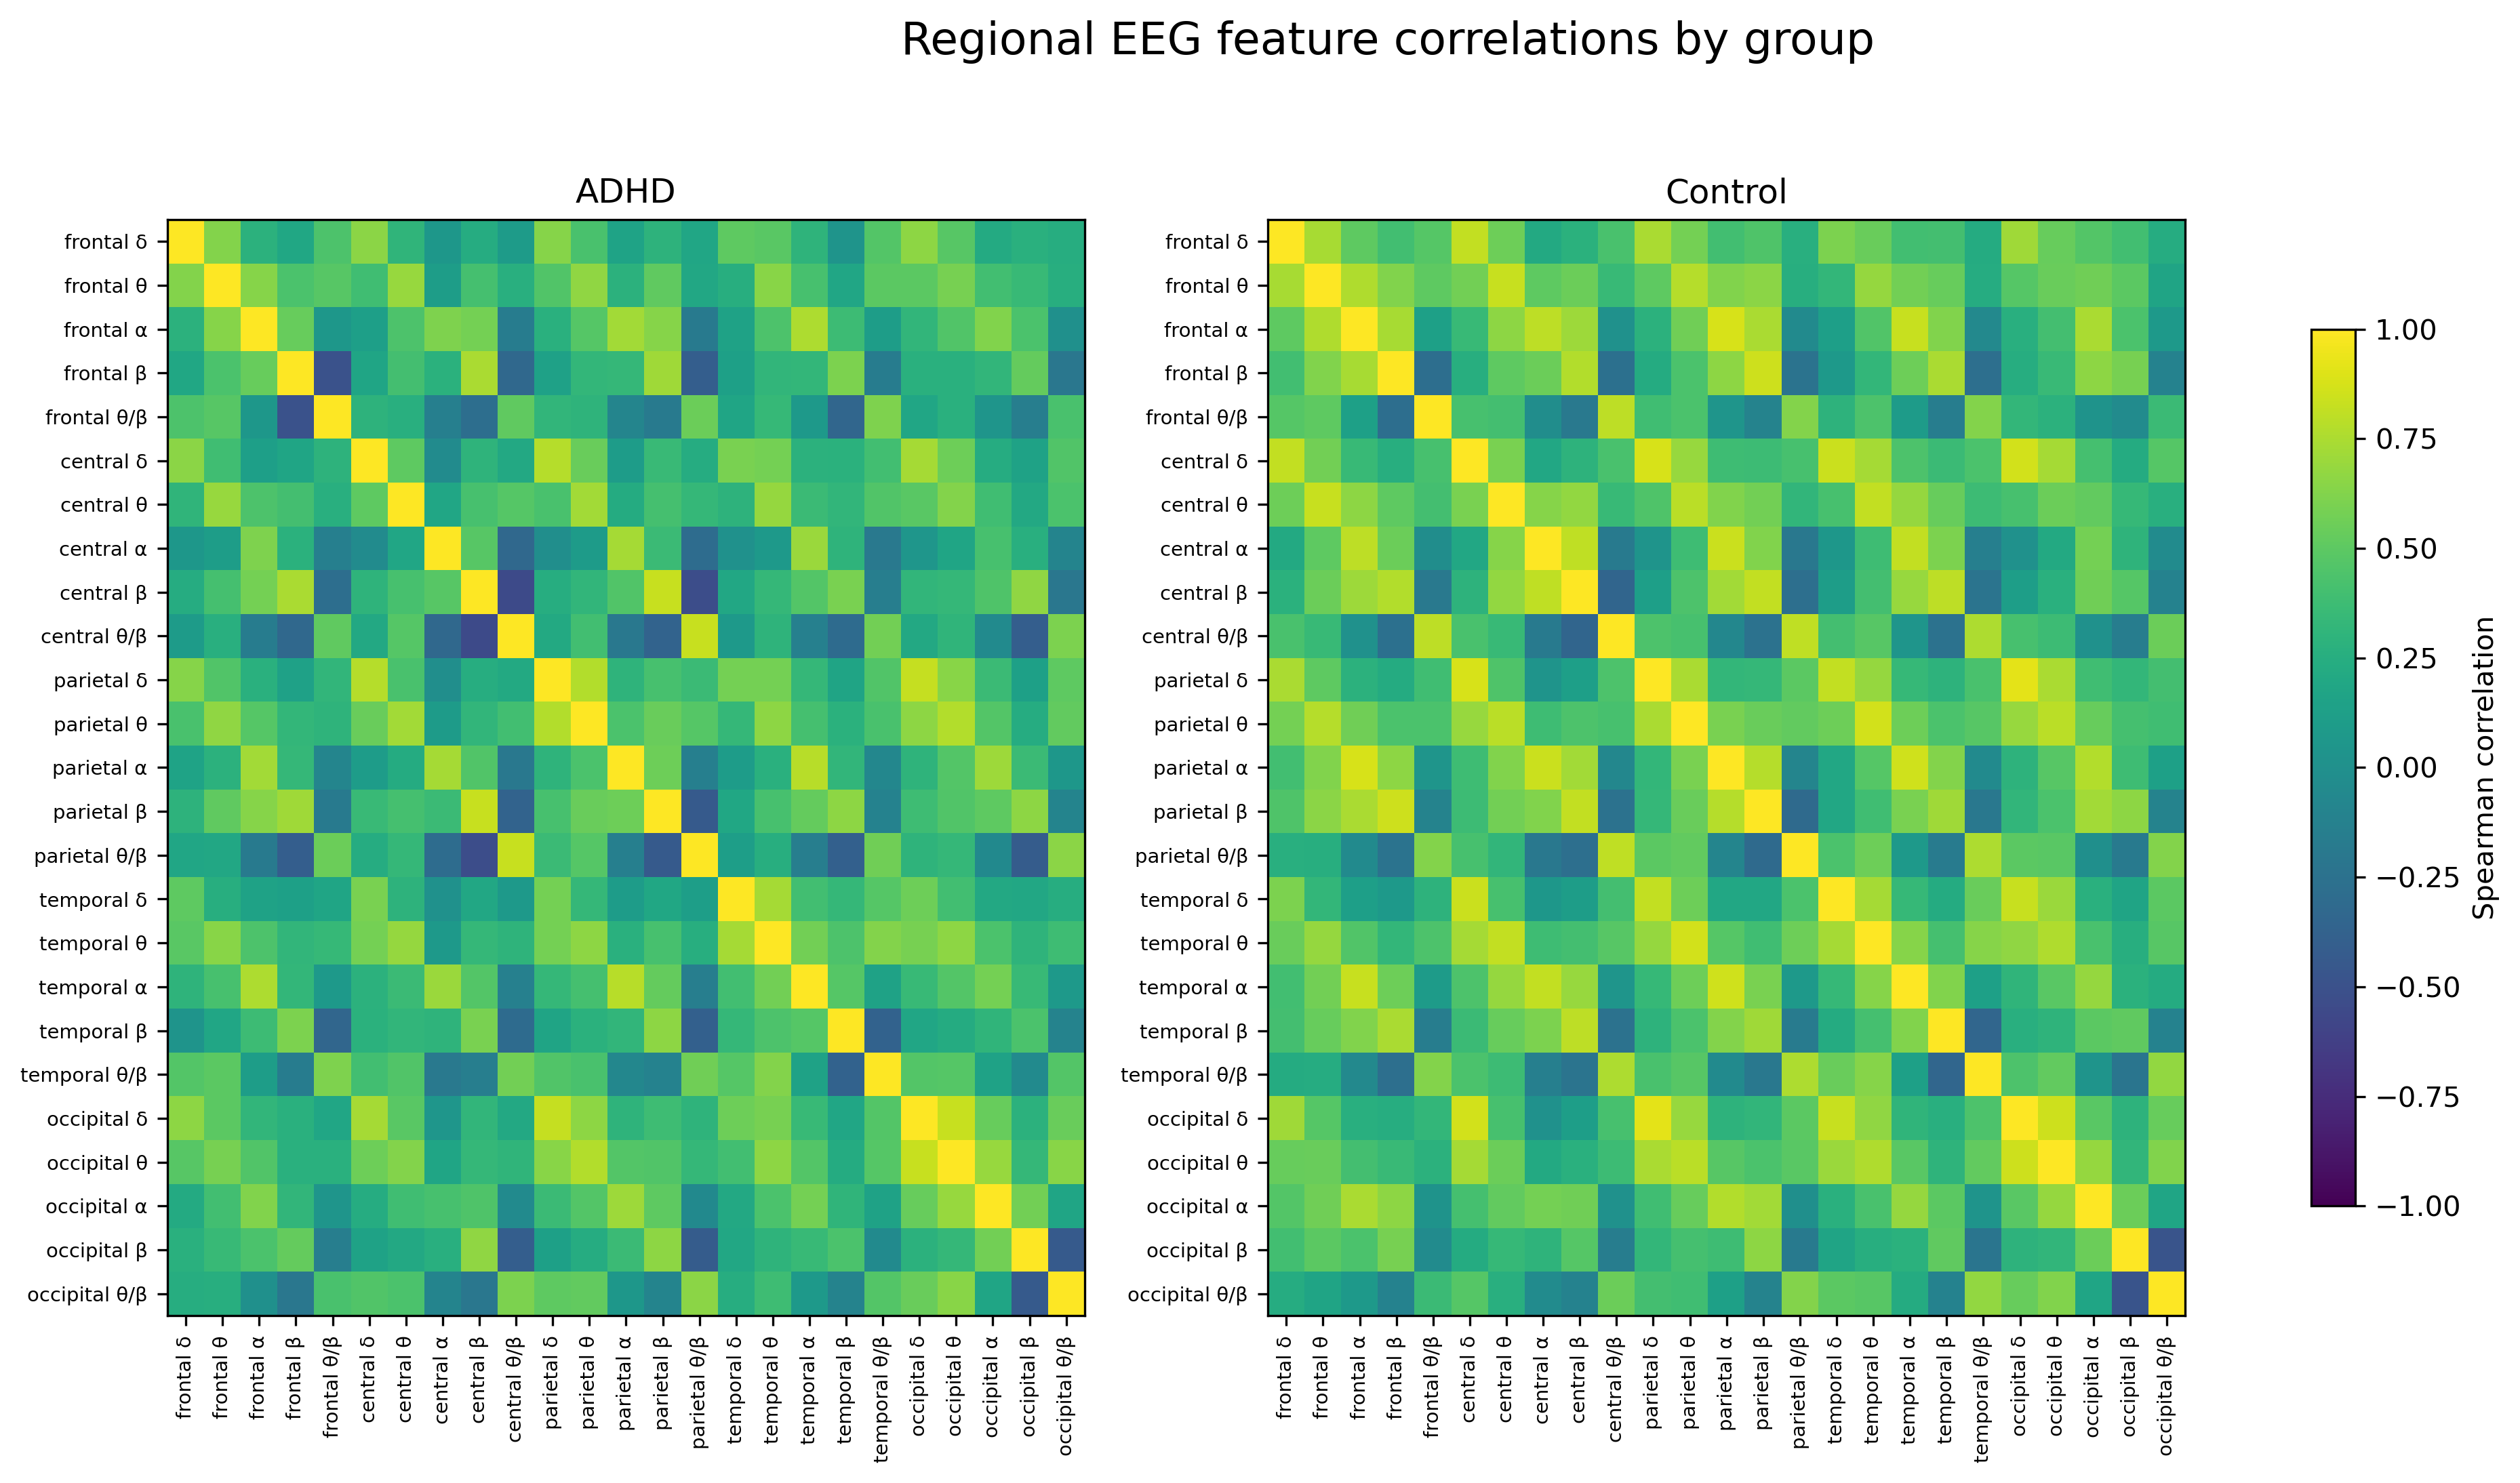
\includegraphics[width=0.98\textwidth]{../figures/1b_regional_correlation_matrix_by_group.png}
	\caption{Matrici di correlazione di Spearman tra feature regionali, calcolate separatamente nei gruppi ADHD e Control.}
	\label{fig:regional_corr_matrix_by_group}
\end{figure}

\begin{table}[H]
	\centering
	\scriptsize
	\begin{tabular}{lllr}
		\hline
		\textbf{Gruppo} & \textbf{Feature 1} & \textbf{Feature 2} & \textbf{$\rho$} \\
		\hline
		ADHD & \texttt{central\_theta\_beta\_ratio} & \texttt{parietal\_theta\_beta\_ratio} & 0.834 \\
		ADHD & \texttt{occipital\_delta\_power\_mean} & \texttt{occipital\_theta\_power\_mean} & 0.830 \\
		ADHD & \texttt{central\_beta\_power\_mean} & \texttt{parietal\_beta\_power\_mean} & 0.830 \\
		ADHD & \texttt{parietal\_delta\_power\_mean} & \texttt{occipital\_delta\_power\_mean} & 0.825 \\
		ADHD & \texttt{parietal\_alpha\_power\_mean} & \texttt{temporal\_alpha\_power\_mean} & 0.788 \\
		ADHD & \texttt{central\_delta\_power\_mean} & \texttt{parietal\_delta\_power\_mean} & 0.779 \\
		ADHD & \texttt{parietal\_theta\_power\_mean} & \texttt{occipital\_theta\_power\_mean} & 0.772 \\
		ADHD & \texttt{parietal\_delta\_power\_mean} & \texttt{parietal\_theta\_power\_mean} & 0.766 \\
		ADHD & \texttt{frontal\_alpha\_power\_mean} & \texttt{temporal\_alpha\_power\_mean} & 0.757 \\
		ADHD & \texttt{frontal\_beta\_power\_mean} & \texttt{central\_beta\_power\_mean} & 0.749 \\
		\hline
		Control & \texttt{parietal\_delta\_power\_mean} & \texttt{occipital\_delta\_power\_mean} & 0.919 \\
		Control & \texttt{frontal\_alpha\_power\_mean} & \texttt{parietal\_alpha\_power\_mean} & 0.881 \\
		Control & \texttt{central\_delta\_power\_mean} & \texttt{parietal\_delta\_power\_mean} & 0.878 \\
		Control & \texttt{central\_delta\_power\_mean} & \texttt{occipital\_delta\_power\_mean} & 0.863 \\
		Control & \texttt{parietal\_theta\_power\_mean} & \texttt{temporal\_theta\_power\_mean} & 0.861 \\
		Control & \texttt{parietal\_alpha\_power\_mean} & \texttt{temporal\_alpha\_power\_mean} & 0.856 \\
		Control & \texttt{occipital\_delta\_power\_mean} & \texttt{occipital\_theta\_power\_mean} & 0.851 \\
		Control & \texttt{frontal\_beta\_power\_mean} & \texttt{parietal\_beta\_power\_mean} & 0.845 \\
		Control & \texttt{central\_delta\_power\_mean} & \texttt{temporal\_delta\_power\_mean} & 0.841 \\
		Control & \texttt{central\_alpha\_power\_mean} & \texttt{parietal\_alpha\_power\_mean} & 0.839 \\
		\hline
	\end{tabular}
	\caption{Dieci correlazioni di Spearman più forti in valore assoluto tra feature regionali, calcolate separatamente nei gruppi ADHD e Control.}
	\label{tab:top_regional_correlations}
\end{table}

Le correlazioni regionali più forti sono positive in entrambi i gruppi. Nel gruppo ADHD la correlazione più elevata riguarda il rapporto theta/beta centrale e parietale, mentre nel gruppo Control la correlazione maggiore riguarda la potenza delta parietale e occipitale.

\subsubsection{Distribuzione delle correlazioni}

Le distribuzioni dei coefficienti di Spearman sono riportate separatamente per feature regionali e canale-livello nelle Figure~\ref{fig:regional_corr_distribution} e~\ref{fig:channel_corr_distribution}.

\begin{figure}[H]
	\centering
	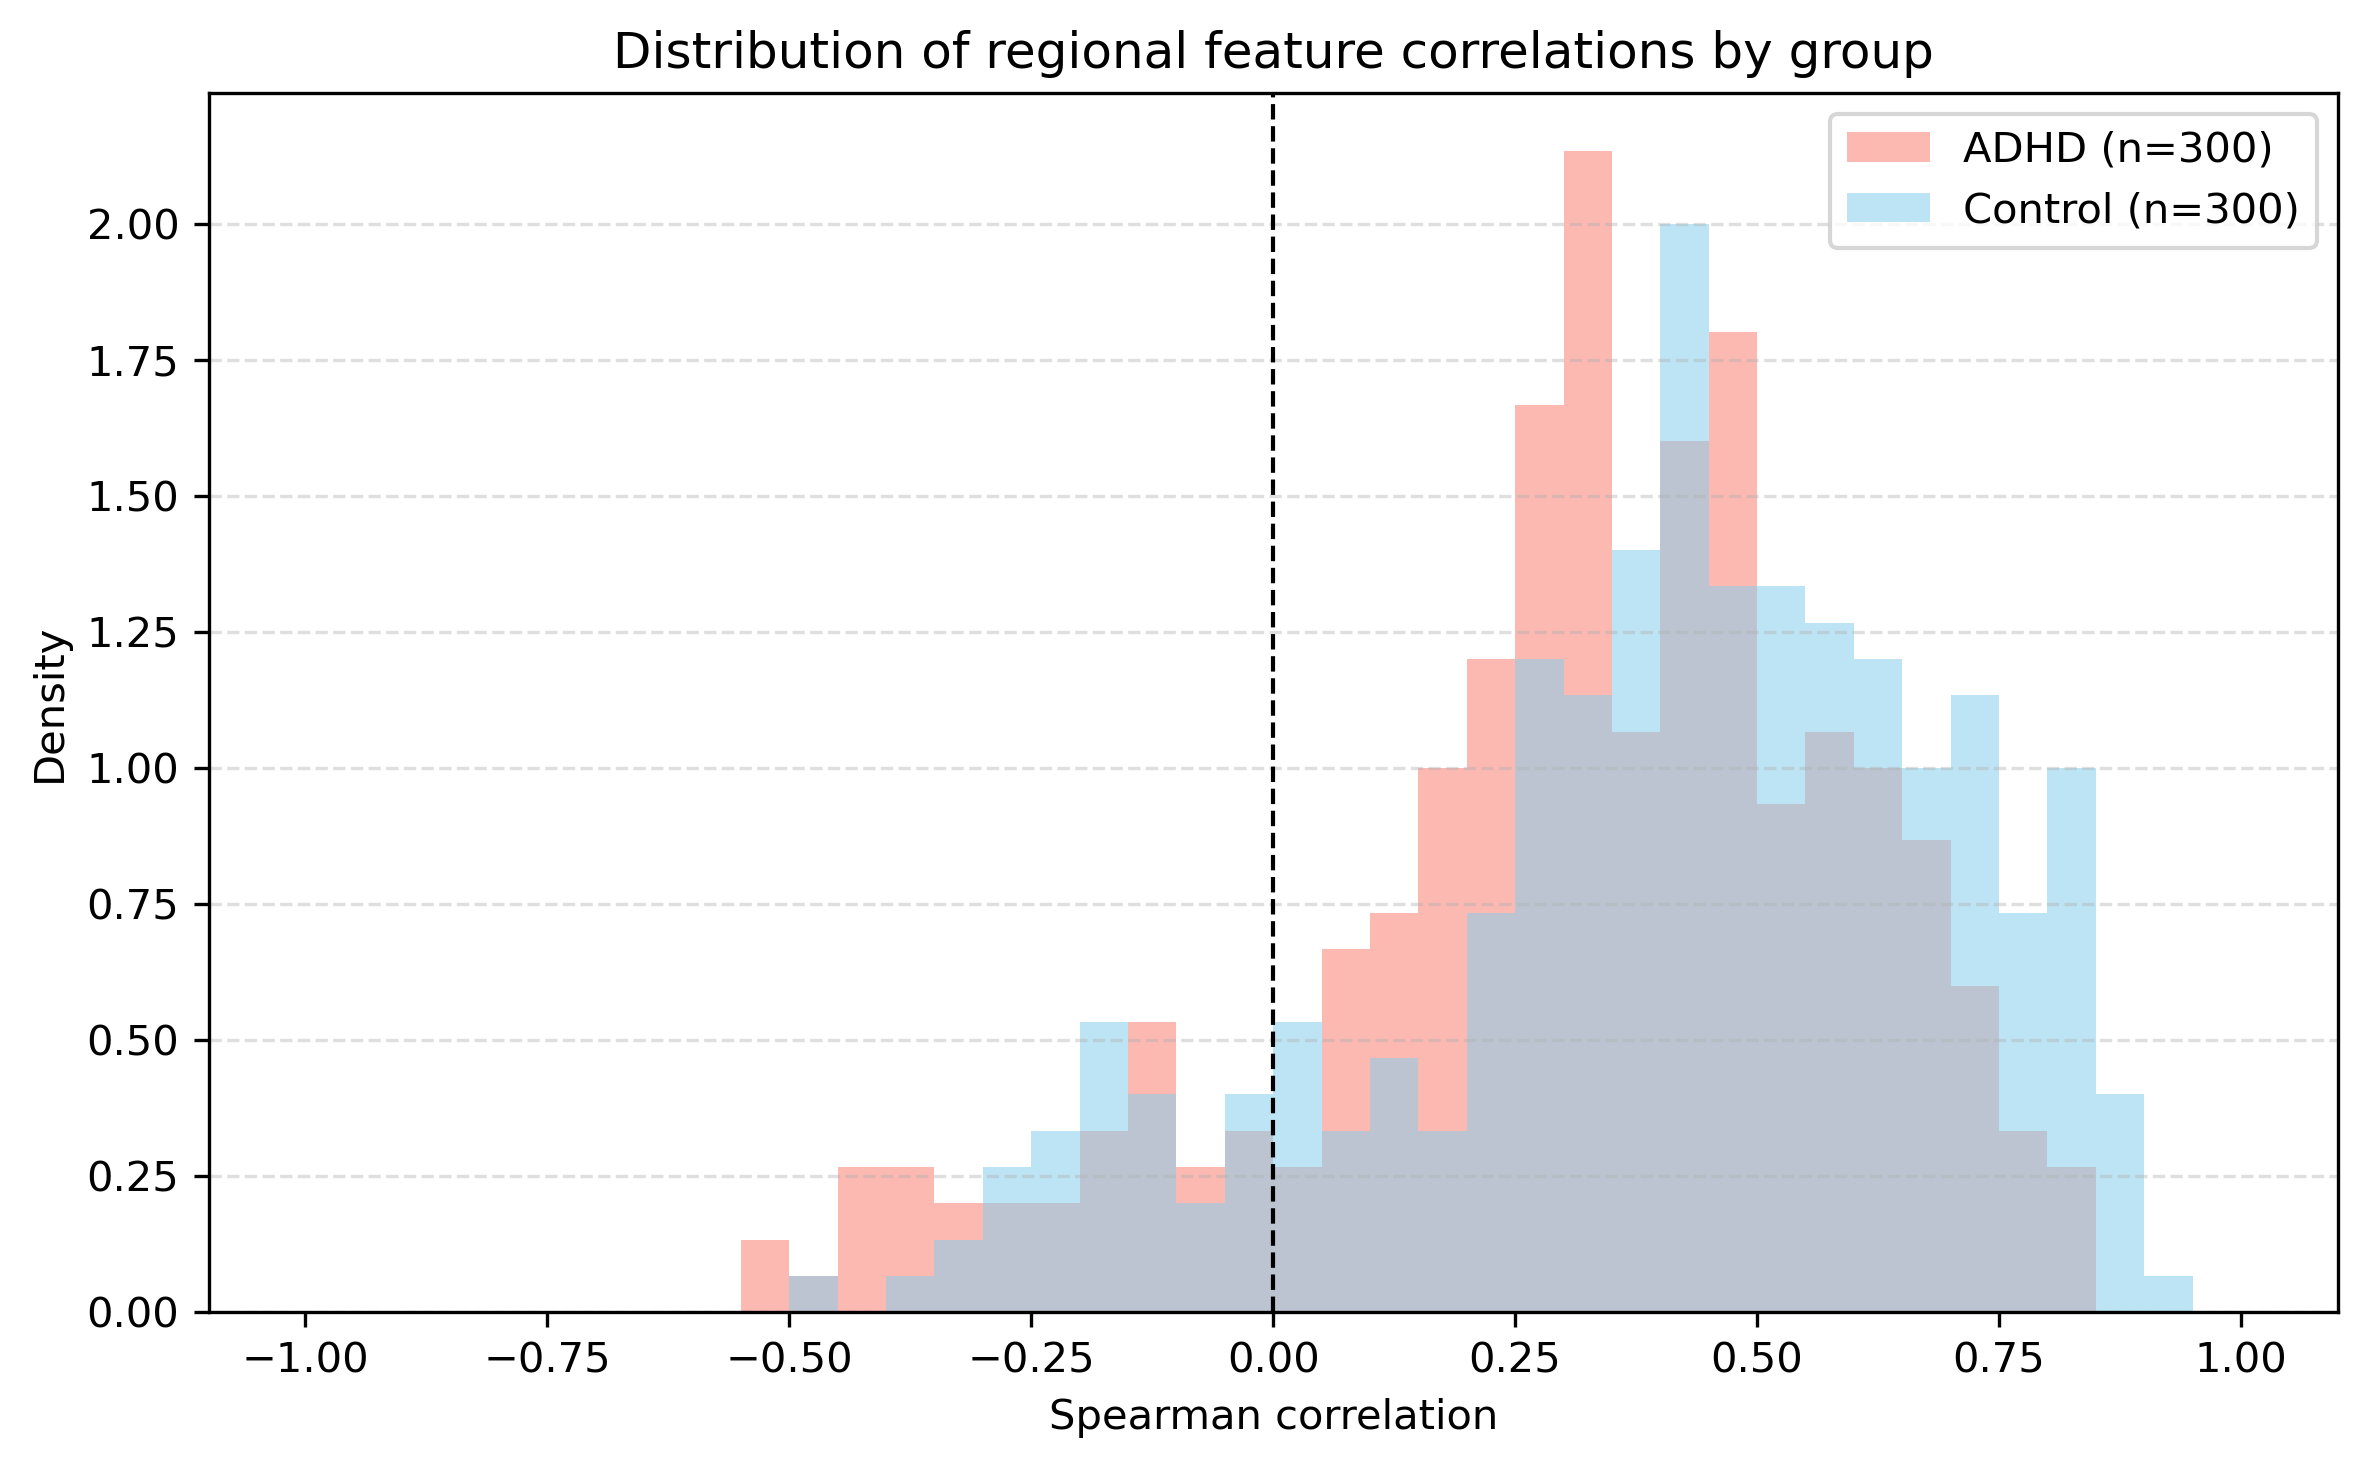
\includegraphics[width=0.85\textwidth]{../figures/1b_regional_correlation_distribution_by_group.png}
	\caption{Distribuzione delle correlazioni di Spearman tra feature regionali, separatamente per ADHD e Control.}
	\label{fig:regional_corr_distribution}
\end{figure}

\begin{figure}[H]
	\centering
	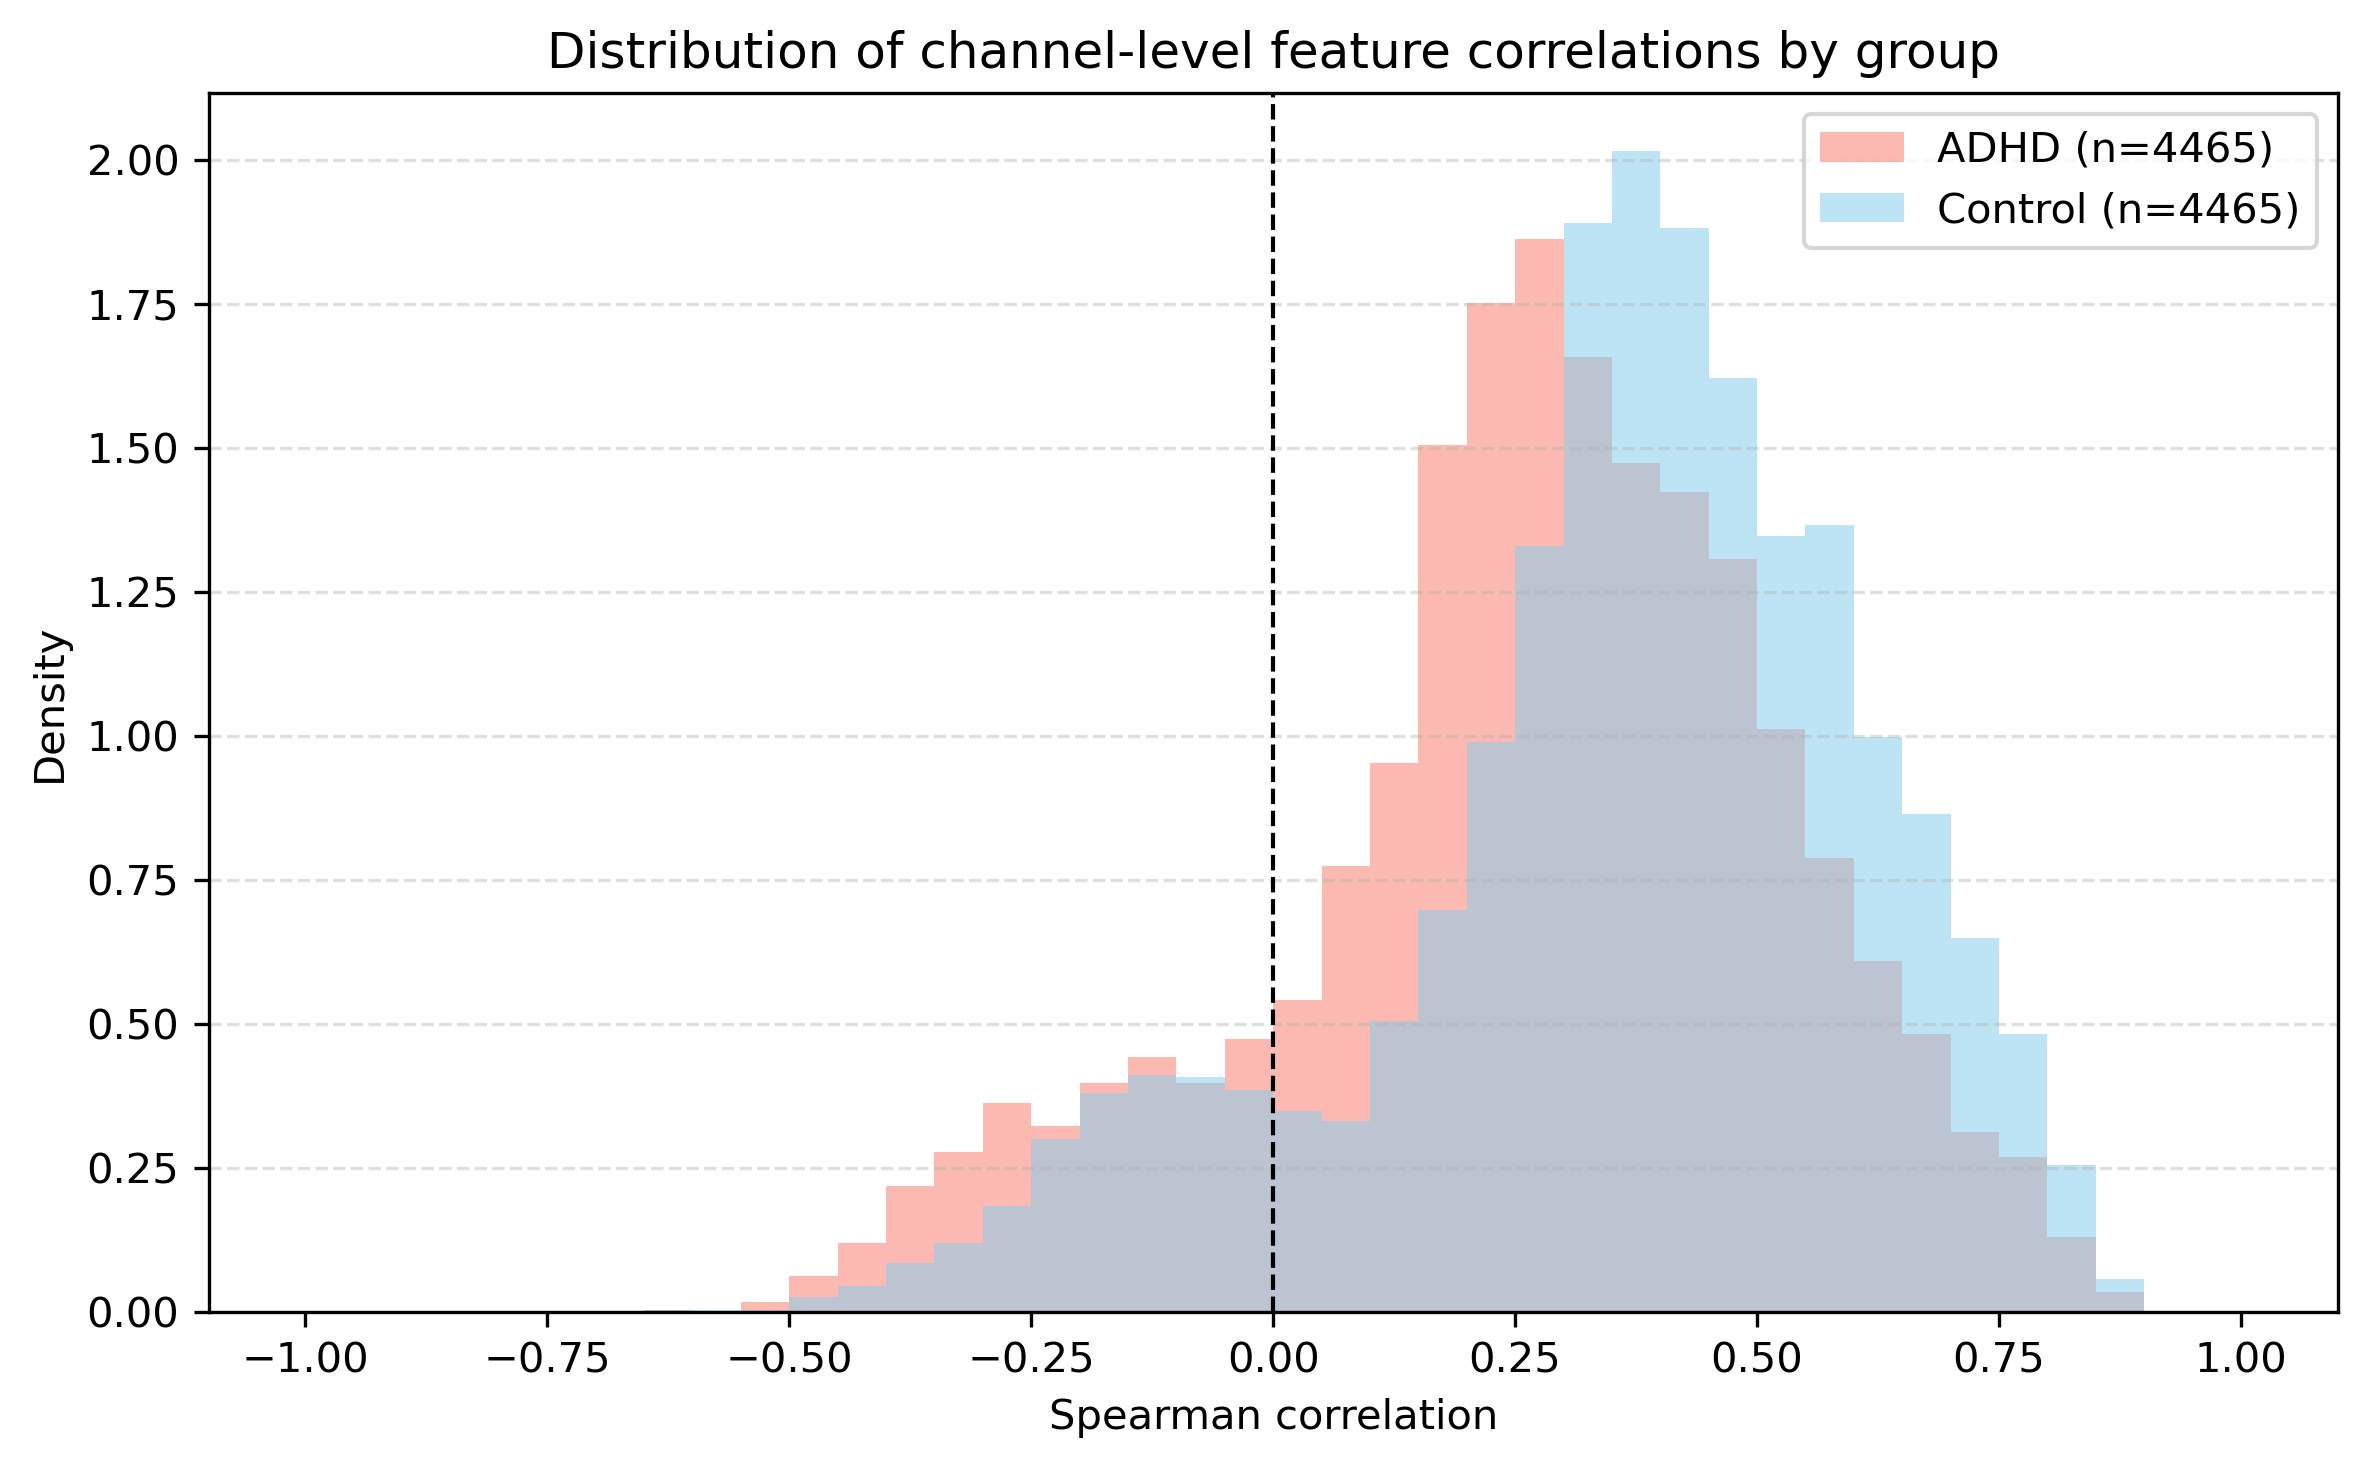
\includegraphics[width=0.85\textwidth]{../figures/1b_channel_correlation_distribution_by_group.png}
	\caption{Distribuzione delle correlazioni di Spearman tra feature canale-livello, separatamente per ADHD e Control.}
	\label{fig:channel_corr_distribution}
\end{figure}

Le distribuzioni mostrano che la maggior parte delle correlazioni è positiva in entrambi i gruppi. Per le feature regionali, il gruppo Control presenta una distribuzione leggermente più spostata verso correlazioni positive elevate, suggerendo una maggiore co-variazione tra feature regionali. Per le feature canale-livello, le distribuzioni dei due gruppi sono più sovrapposte, anche se il gruppo Control mantiene una coda più estesa verso valori positivi alti.

\subsection{Classificazione Random Forest}

Per valutare il contenuto predittivo delle feature EEG, è stato addestrato un classificatore Random Forest. Sono stati confrontati tre set di feature: tutte le feature EEG, le sole feature canale-livello e le sole feature regionali. Il confronto è stato eseguito mediante cross-validation stratificata a 5 fold sul training/validation set.

\begin{table}[H]
	\centering
	\small
	\begin{tabular}{llllllll}
		\hline
		\textbf{Feature set} & \textbf{N} & \textbf{Accuracy} & \textbf{Balanced acc.} & \textbf{Precision} & \textbf{Recall} & \textbf{F1} & \textbf{ROC-AUC} \\
		\hline
		All & 120 & 0.676 & 0.677 & 0.660 & 0.751 & 0.699 & 0.674 \\
		Channel-level & 95 & 0.614 & 0.610 & 0.604 & 0.707 & 0.646 & 0.681 \\
		Regional mean & 25 & 0.676 & 0.678 & 0.670 & 0.749 & 0.700 & 0.729 \\
		\hline
	\end{tabular}
	\caption{Confronto delle performance medie in cross-validation per i tre insiemi di feature testati con Random Forest.}
	\label{tab:rf_feature_set_comparison}
\end{table}

\begin{figure}[H]
	\centering
	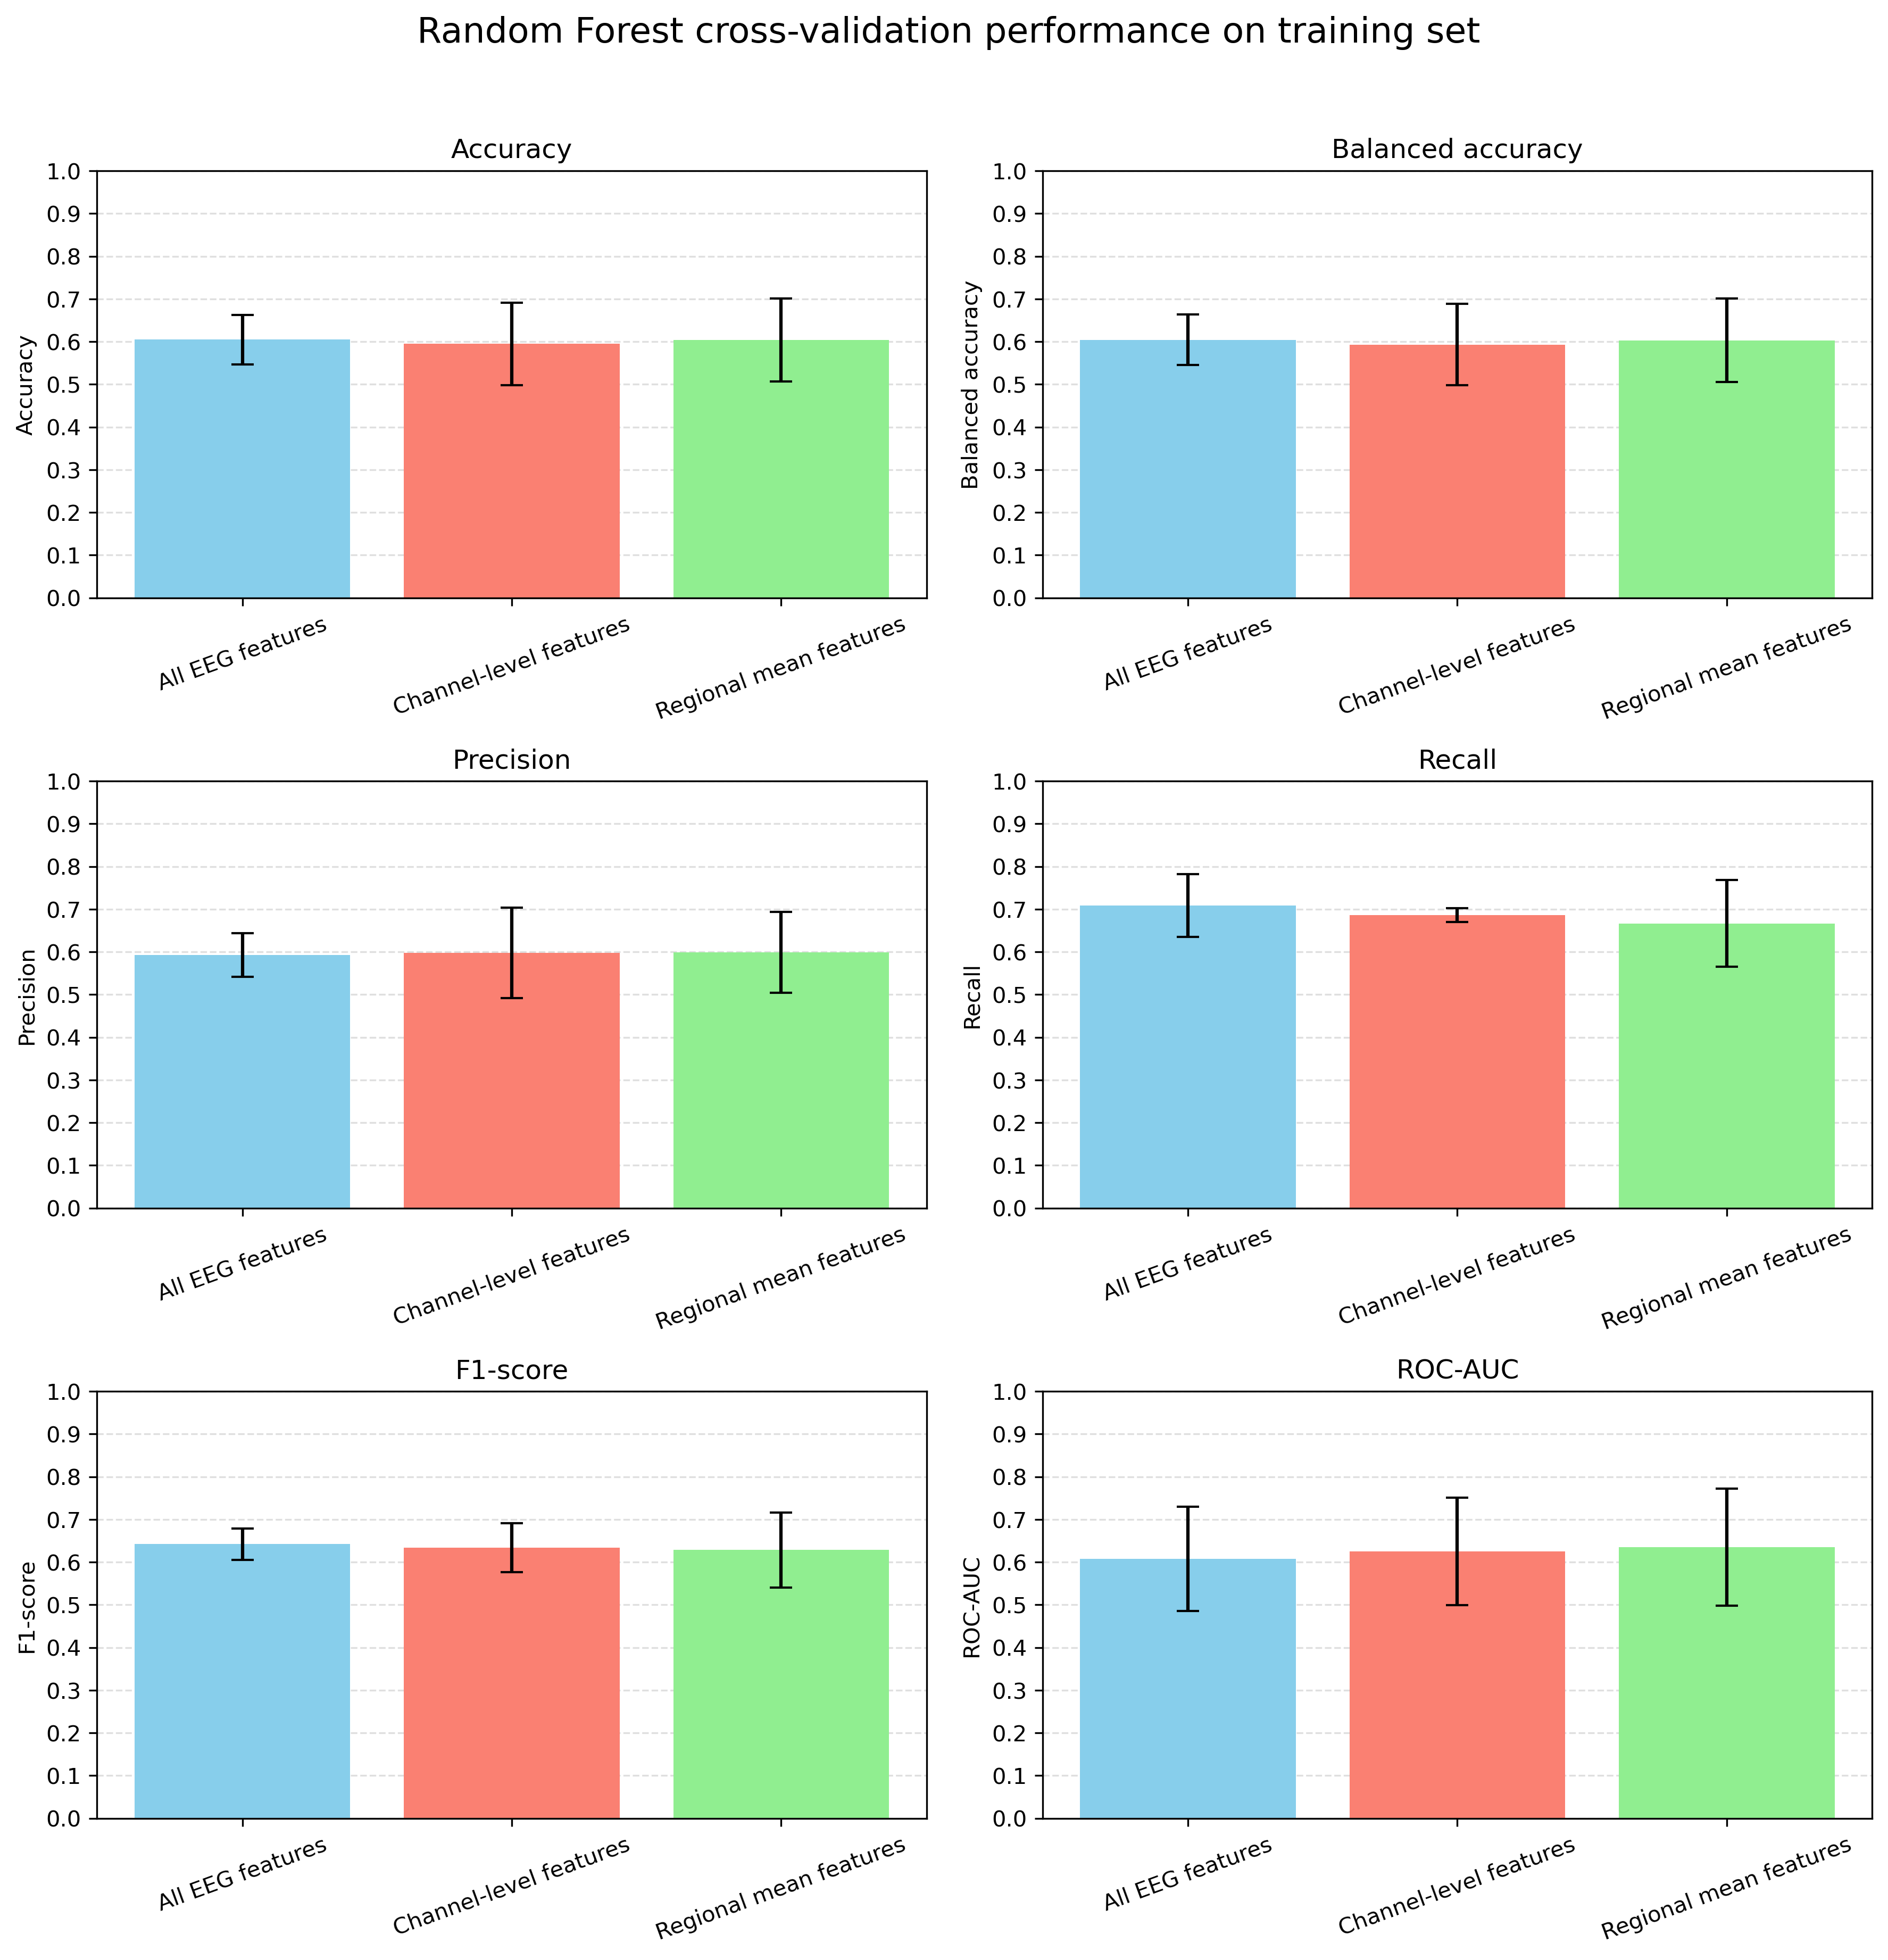
\includegraphics[width=0.95\textwidth]{../figures/2a_rf_feature_set_comparison.png}
	\caption{Confronto delle metriche di cross-validation del modello Random Forest per i tre insiemi di feature.}
	\label{fig:rf_feature_set_comparison}
\end{figure}

Le feature regionali ottengono la migliore balanced accuracy media. Le differenze rispetto all'insieme completo non sono ampie, ma il risultato suggerisce che una rappresentazione regionale sia sufficiente a conservare informazione discriminativa, riducendo così la dimensionalità rispetto alle feature relative ai canali singoli.

\subsection{Performance del modello finale}

Il modello finale, dopo tunng sui parametri ha mostrato performance migliori con parametri: 
\begin{table}
\begin{tabular}{ll}
	\hline
	\textbf{Iperparametro} & \textbf{Valori ottimali} \\
	\hline
	\texttt{n\_estimators} & \text{3000} \\
	\texttt{max\_depth} & \text{None0} \\
	\texttt{min\_samples\_leaf} & 1 \\
	\texttt{max\_features} & \text{log2} \\
	\hline
\end{tabular}
\caption{Iperparametri ottimali Random Forest su features regionali.}
\end{table}

È stato addestrato sull'intero training/validation set utilizzando le feature regionali, ed è stato valutato sul test set indipendente. Le metriche finali sono riportate nella Tabella~\ref{tab:rf_final_metrics}.

\begin{table}[H]
	\centering
	\small
	\begin{tabular}{lr}
		\hline
		\textbf{Metrica} & \textbf{Valore} \\
		\hline
		Feature set & Regional mean features \\
		N feature & 25 \\
		Accuracy & 0.760 \\
		Balanced accuracy & 0.756 \\
		Precision & 0.733 \\
		Recall & 0.846 \\
		F1-score & 0.786 \\
		ROC-AUC & 0.717 \\
		\hline
	\end{tabular}
	\caption{Metriche finali del modello Random Forest valutato sul test set indipendente.}
	\label{tab:rf_final_metrics}
\end{table}

\begin{figure}[H]
	\centering
	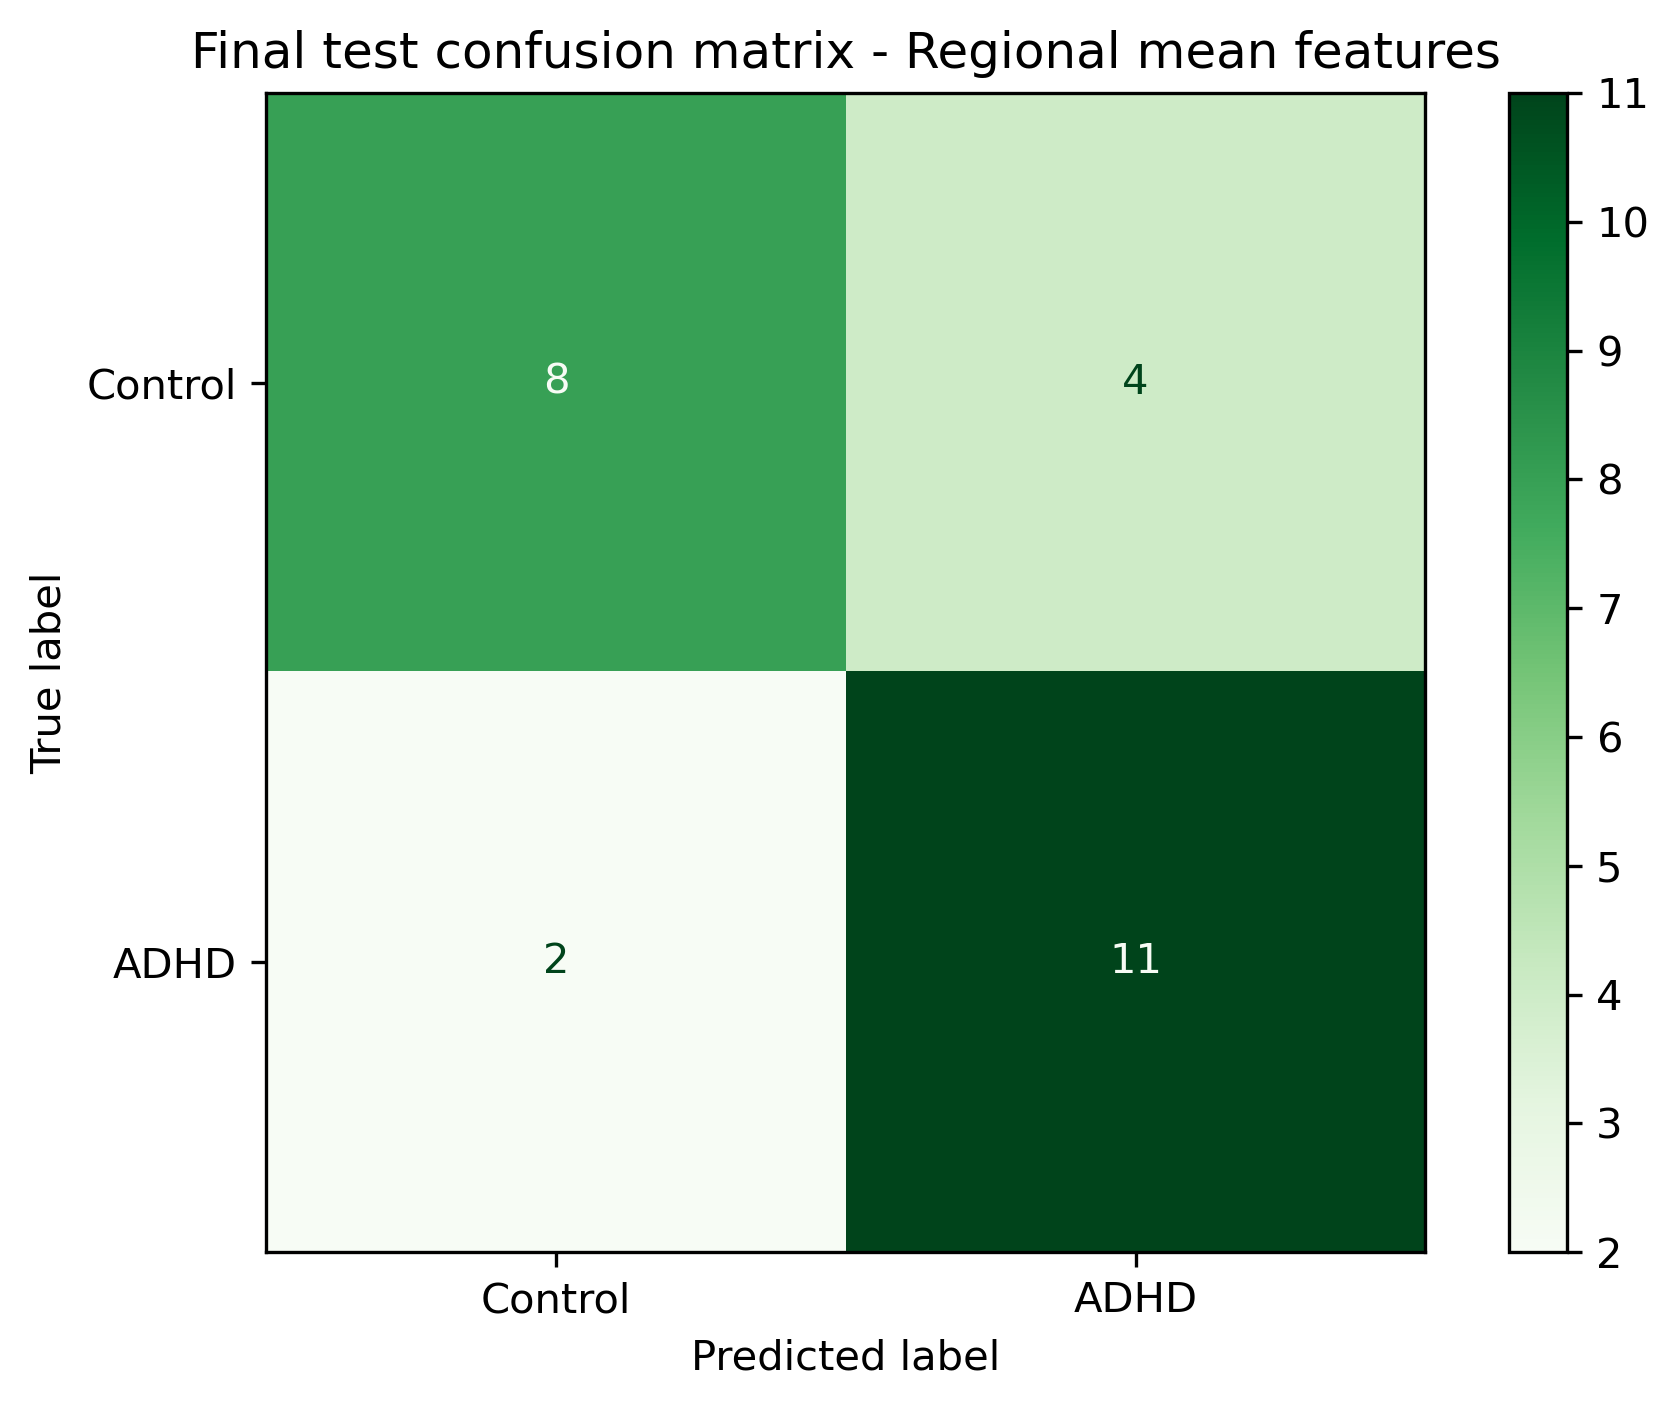
\includegraphics[width=0.60\textwidth]{../figures/2a_rf_best_feature_set_confusion_matrix.png}
	\caption{Confusion matrix del modello Random Forest finale valutato sul test set indipendente.}
	\label{fig:rf_confusion_matrix}
\end{figure}

La confusion matrix mostra 8 soggetti Control correttamente classificati su 12 e 11 soggetti ADHD correttamente classificati su 13. Gli errori sono costituiti da 4 falsi positivi e 2 falsi negativi. Il modello presenta quindi un recall elevato per la classe ADHD, ma una specificità più limitata per la classe Control.

La capacità discriminativa del modello finale è stata valutata anche tramite curva ROC.

\begin{figure}[H]
	\centering
	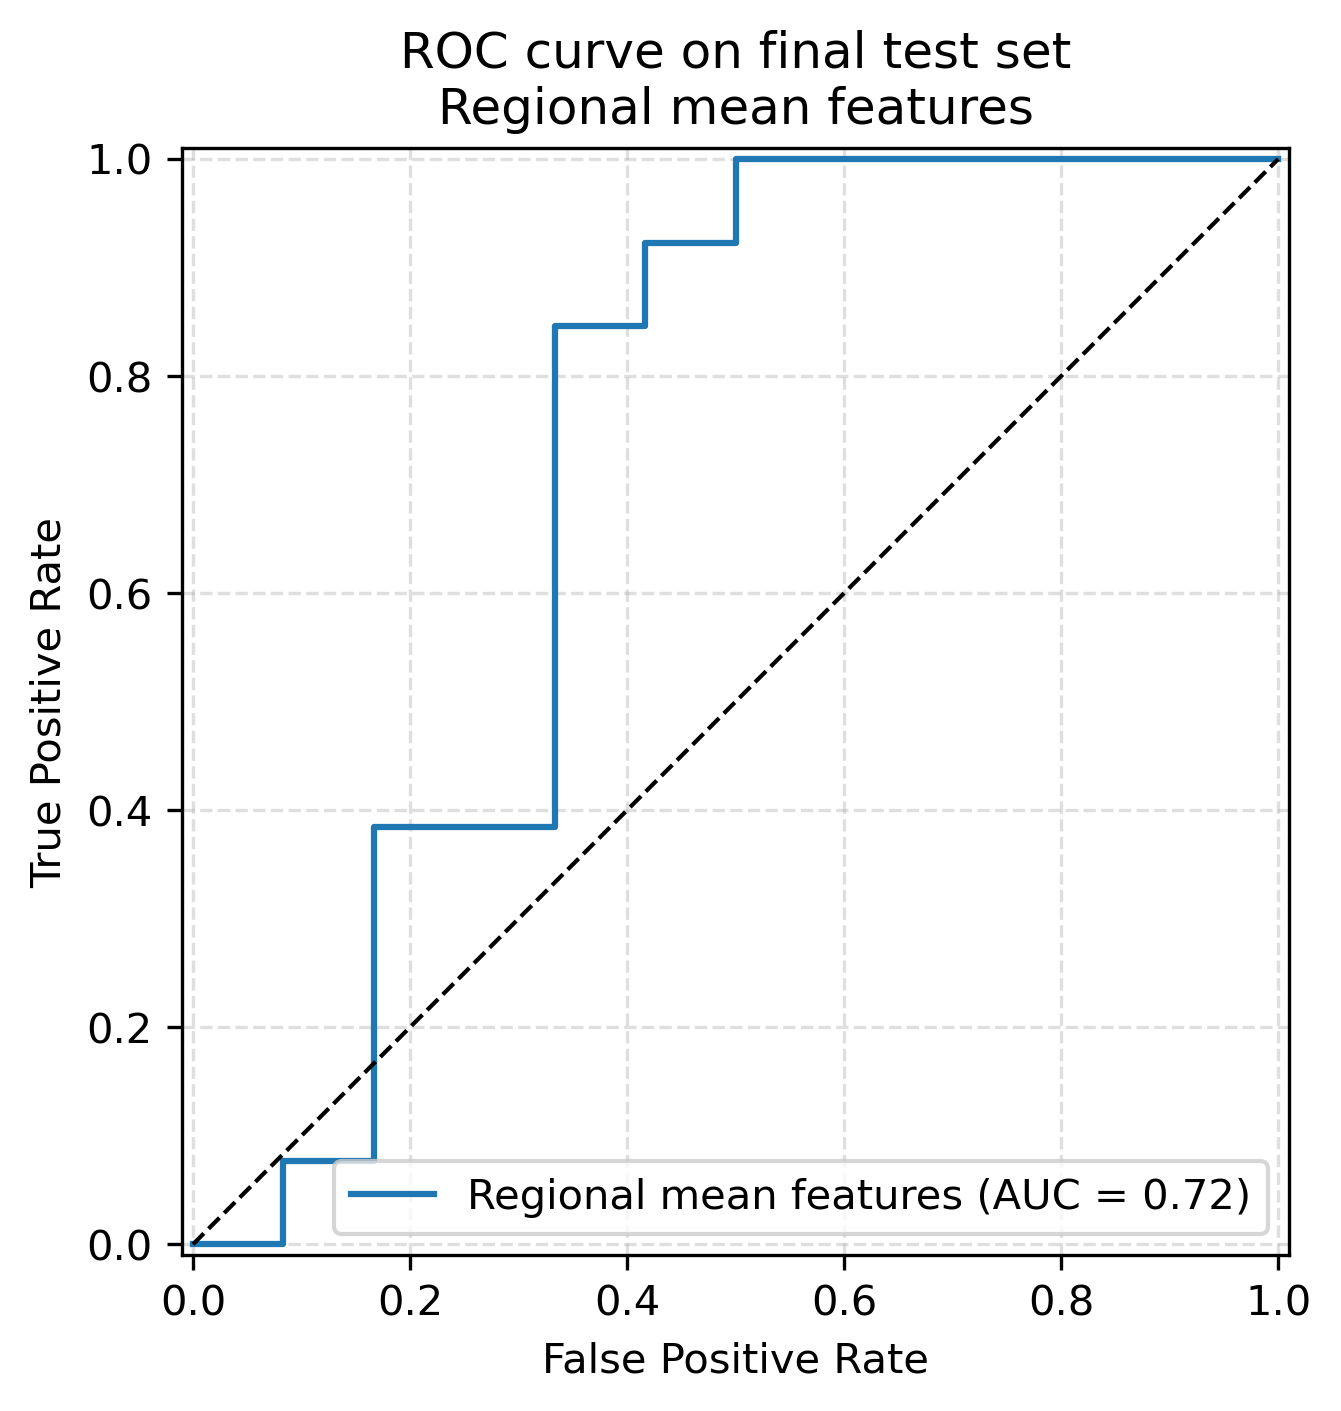
\includegraphics[width=0.60\textwidth]{../figures/2a_rf_best_feature_set_roc_curve.png}
	\caption{Curva ROC del modello Random Forest finale sul test set indipendente. La linea tratteggiata rappresenta la performance casuale.}
	\label{fig:rf_roc_curve}
\end{figure}

La curva ROC mostra una capacità di separazione superiore al caso casuale. Il valore di ROC-AUC ottenuto sul test set è pari a 0.72 come già indicato in \ref{tab:rf_final_metrics}. 


\subsection{Feature importance}

La feature importance della Random Forest è stata utilizzata per identificare le variabili maggiormente coinvolte nella classificazione. Le dieci feature più importanti sono riportate in Figura~\ref{fig:rf_feature_importance}.

\begin{figure}[H]
	\centering
	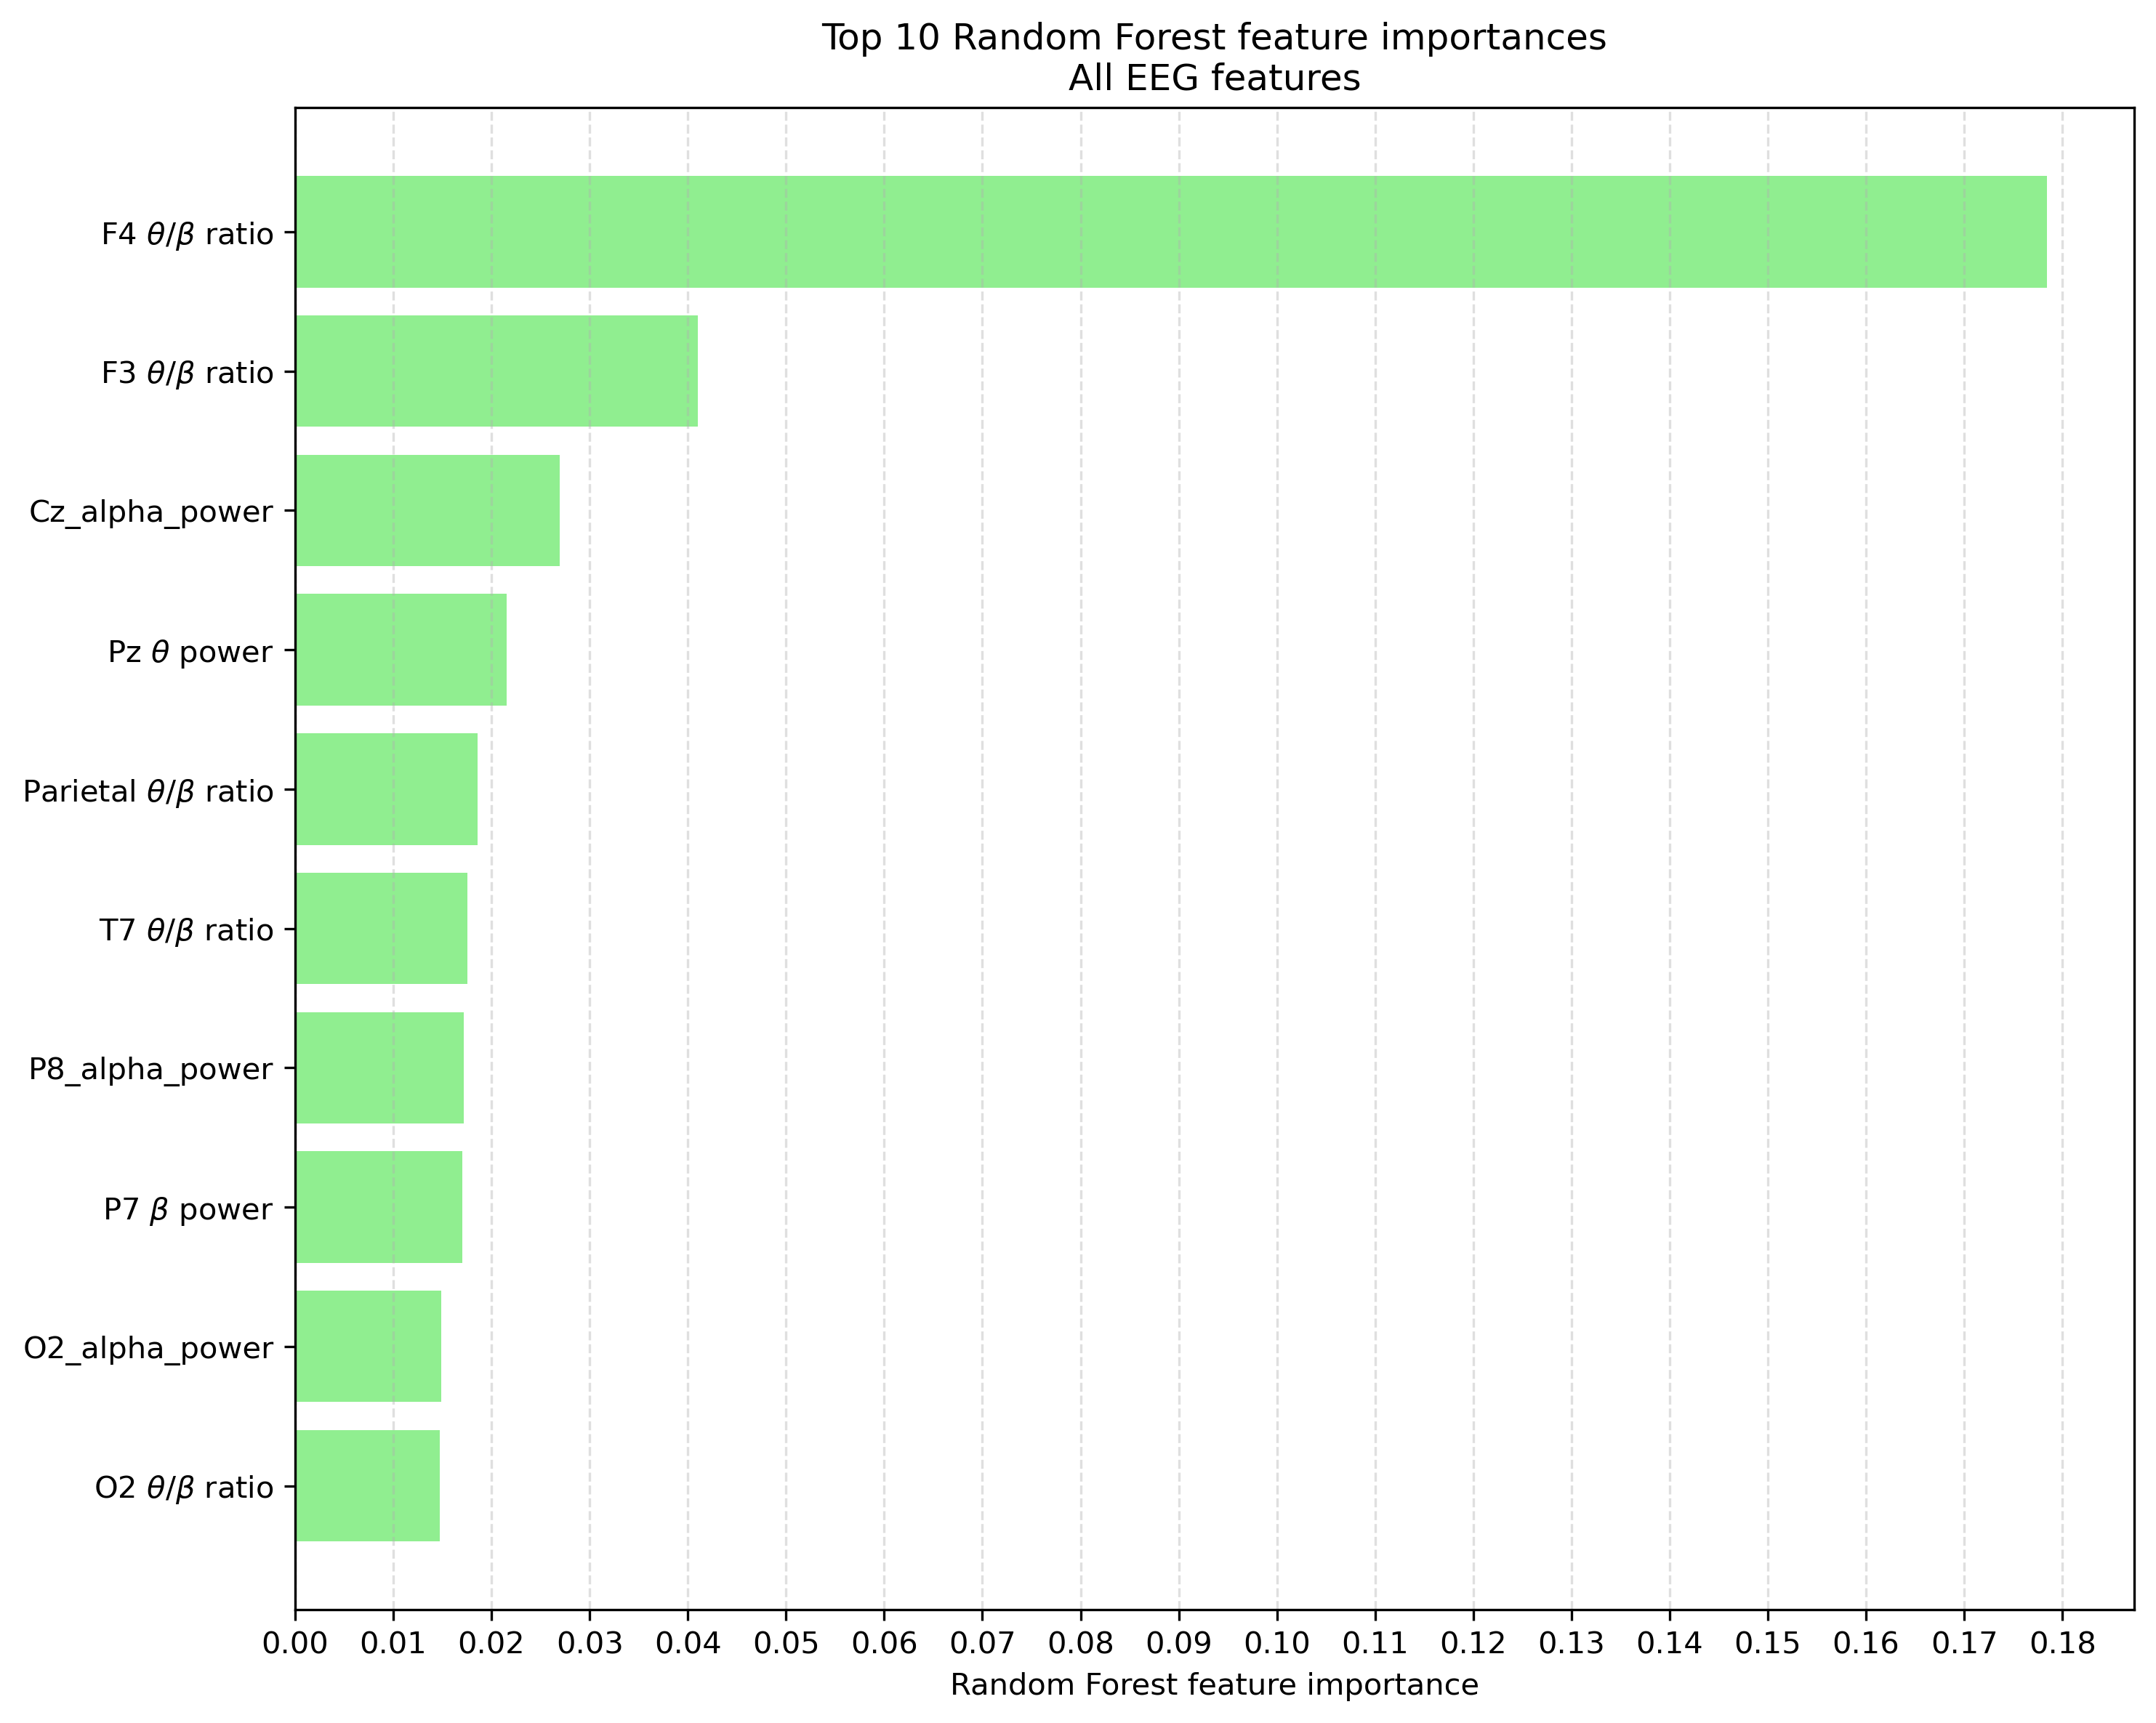
\includegraphics[width=0.85\textwidth]{../figures/2a_rf_best_feature_set_feature_importance_top10.png}
	\caption{Prime dieci feature più importanti secondo il modello Random Forest finale.}
	\label{fig:rf_feature_importance}
\end{figure}

La feature più importante è il rapporto theta/beta temporale, coerentemente con l'analisi statistica, in cui la stessa feature presentava il maggiore effect size assoluto. Tra le altre feature rilevanti compaiono potenze di banda centrali, parietali e occipitali.

Per valutare la ridondanza tra le feature maggiormente utilizzate dal modello, è stata calcolata la matrice di correlazione di Spearman tra le dieci feature con maggiore feature importance.

\begin{figure}[H]
	\centering
	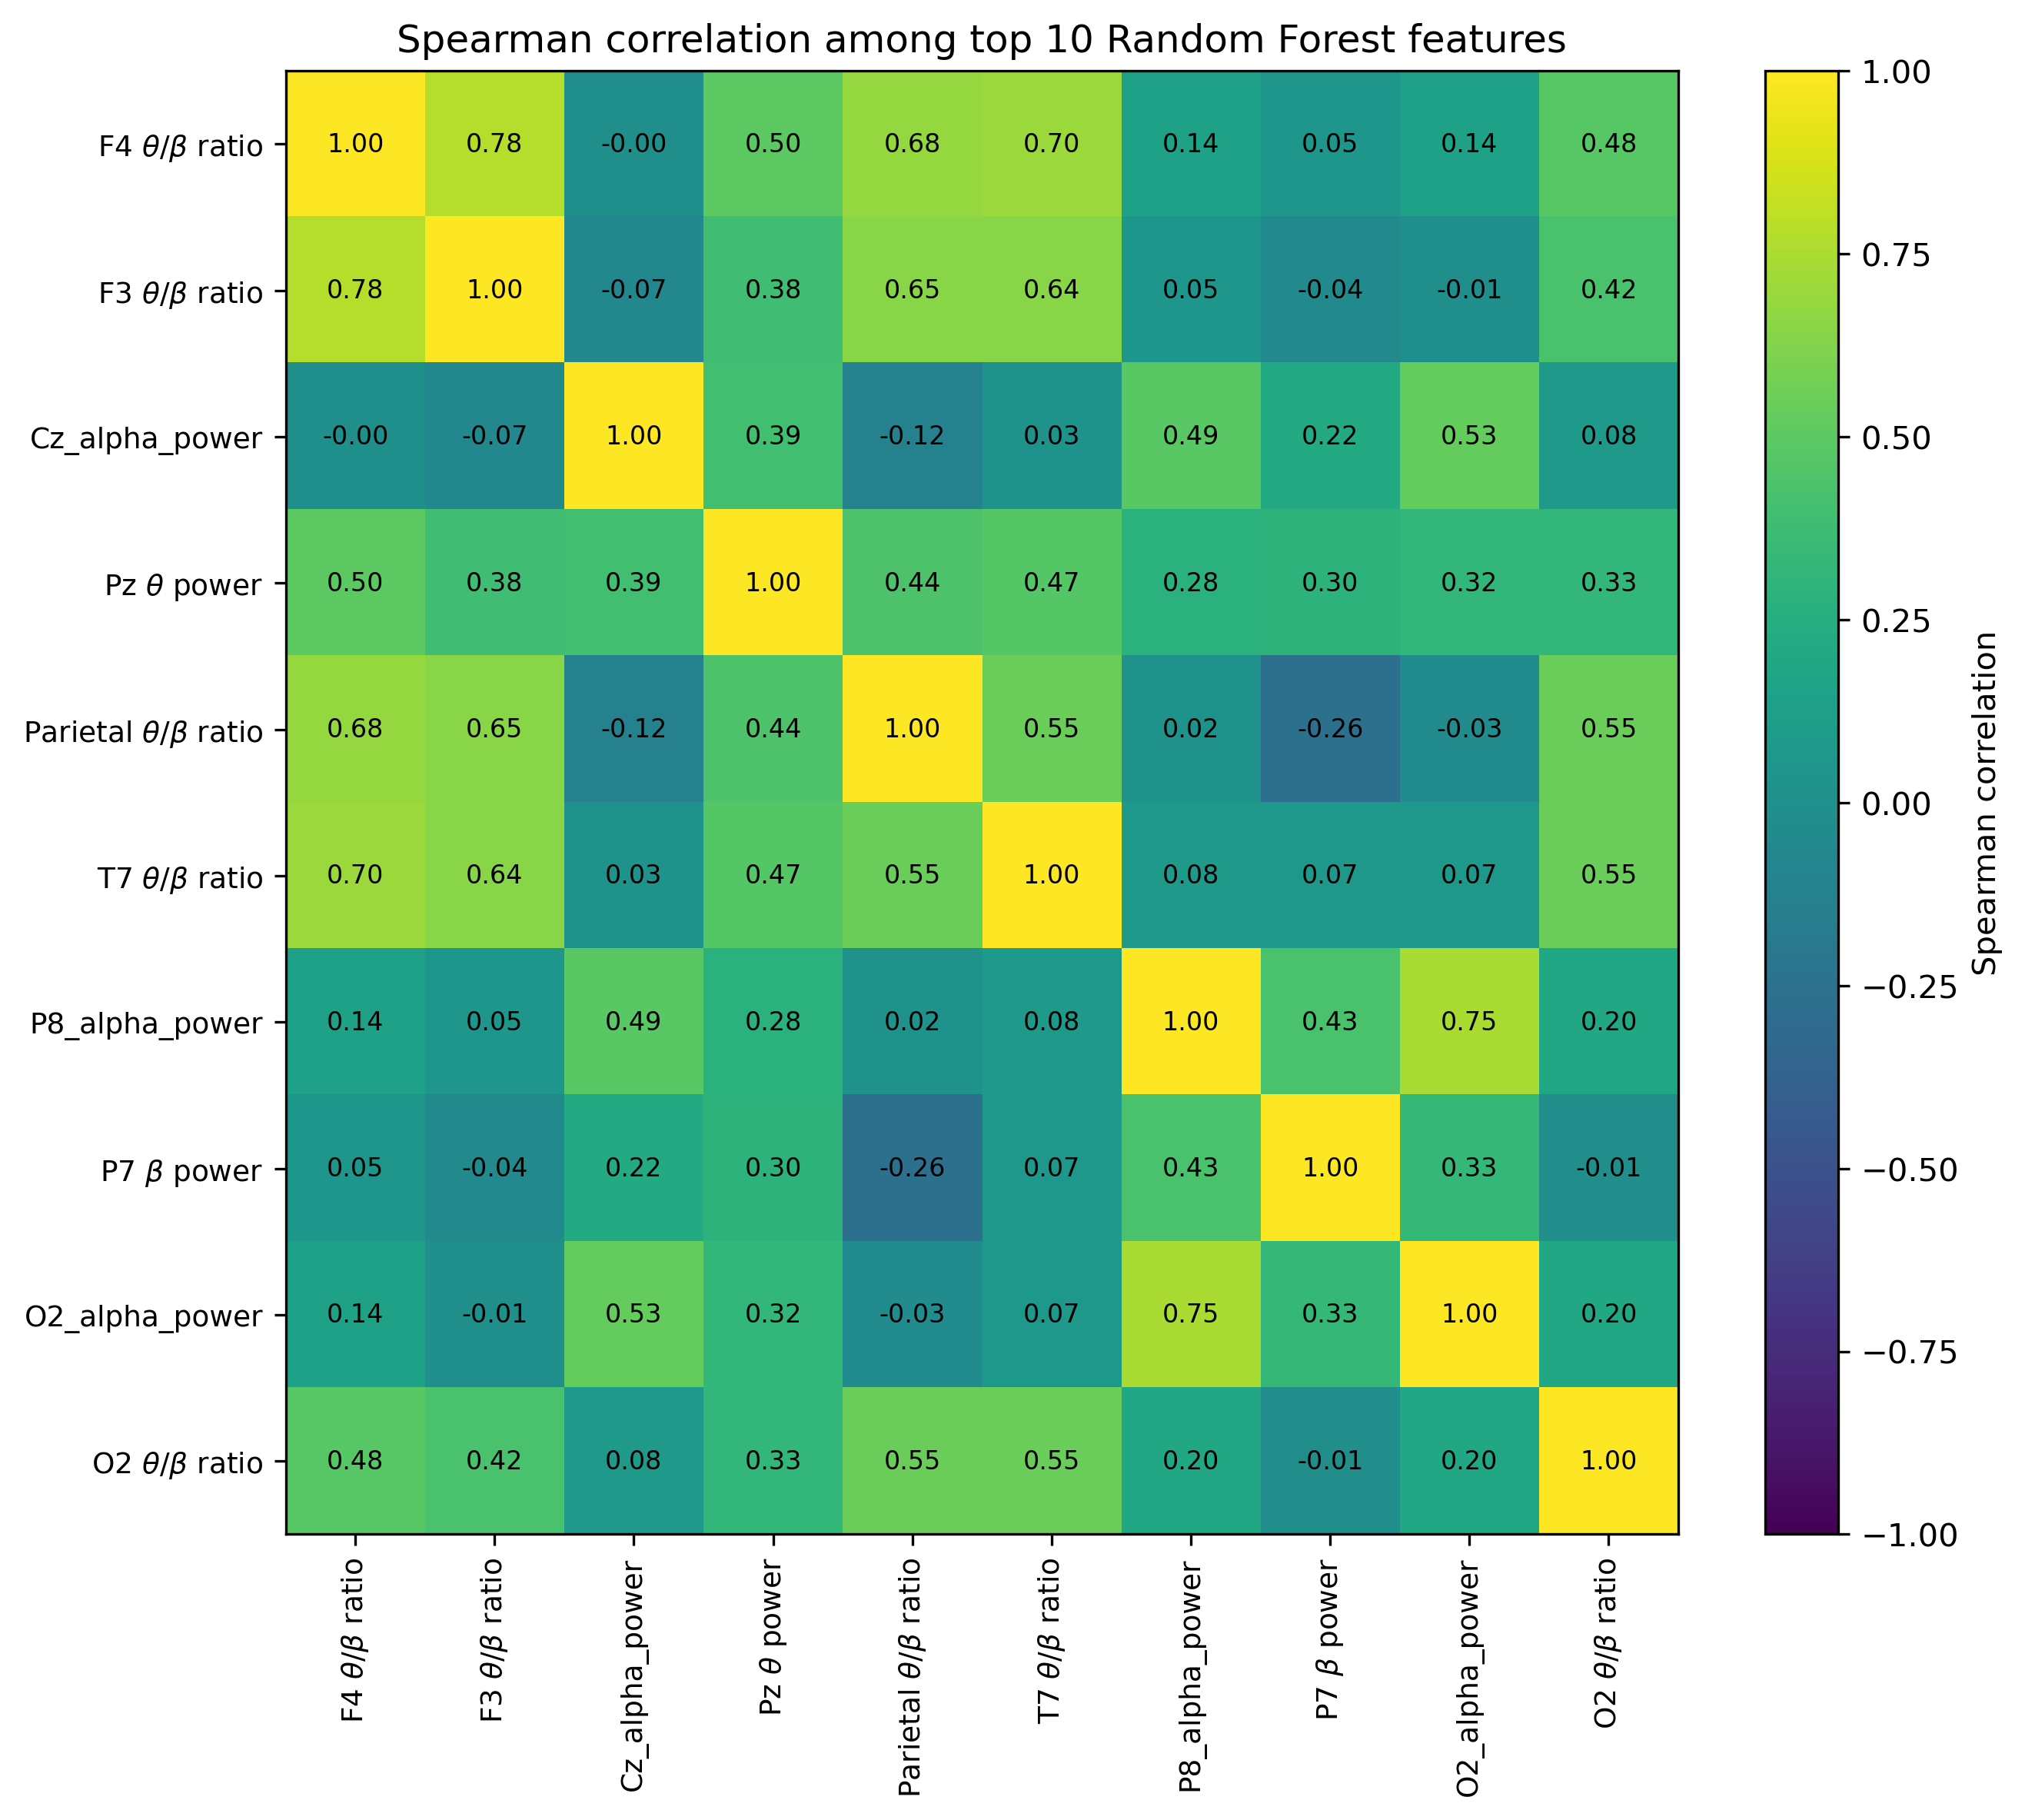
\includegraphics[width=0.85\textwidth]{../figures/2a_rf_top10_feature_importance_correlation_matrix.png}
	\caption{Matrice di correlazione di Spearman tra le dieci feature più importanti secondo la Random Forest.}
	\label{fig:rf_top10_importance_corr}
\end{figure}

La matrice mostra che diverse feature importanti sono tra loro correlate. Questo indica che il modello non utilizza dieci feature completamente indipendenti, ma un insieme di variabili parzialmente ridondanti che descrivono aspetti correlati dell'attività spettrale regionale.


